\documentclass[aspectratio=169]{beamer}

% Document metadata

\subtitle{ELEC0447 - Analysis of electric power and energy systems}
\title{Frequency control}
\author[BC]{Bertrand Cornélusse}
\institute{University of Liège}
\date{Academic Year 2026--2027}

% Image for the title page (use include graphics option to properly size/place it)
\titlegraphic{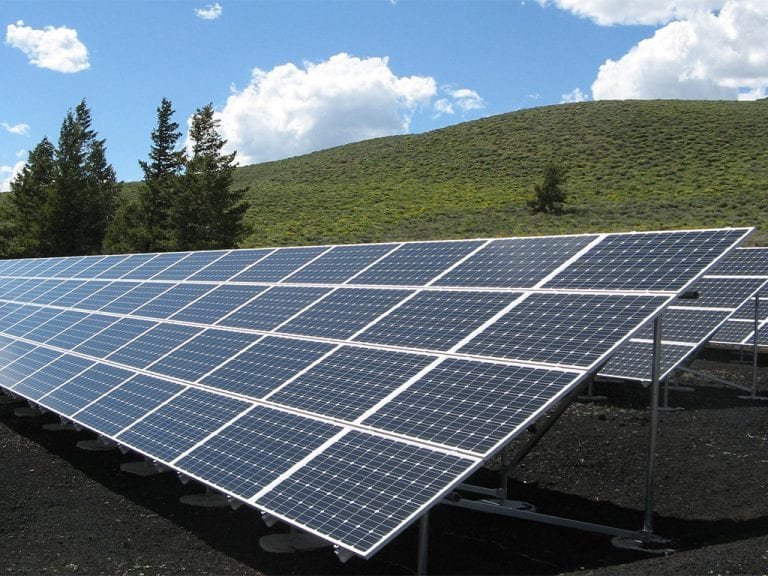
\includegraphics[height=\paperheight]{banner.jpg}}
\usetheme[titlestyle=style1]{trigon}
%\usetheme[sectionstyle=style2]{trigon}

% Define logos to use (comment if no logo)
\biglogo{uliege_faculte_sciencesappliquees_logo_rvb_pos.pdf} % Used on titlepage only
\smalllogo{} % Used on top right corner of regular frames

% ------ If you want to change the theme default colors, do it here ------
%\definecolor{tPrim}{HTML}{00843B}   % Green
%\definecolor{tSec}{HTML}{289B38}    % Green light
%\definecolor{tAccent}{HTML}{F07F3C} % Orange

% ------ Packages and definitions used for this demo. Can be removed ------
\usepackage{appendixnumberbeamer} % To use \appendix command
\pdfstringdefDisableCommands{% Fix hyperref translate warning with \appendix
\def\translate#1{#1}%
}
\usepackage{pgf-pie} % For pie charts
\usepackage{caption} % For subfigures
\usepackage{subcaption} % For subfigures
\usepackage{xspace}
\newcommand{\themename}{\textbf{\textsc{trigon}}\xspace}
\usepackage[scale=2]{ccicons} % Icons for CC-BY-SA
\usepackage{booktabs} % Better tables
\usepackage{amsmath}
\usepackage{amssymb}
\usepackage{amsfonts}
\usepackage{algorithm}
\usepackage{algpseudocodex}
\usepackage{multicol}
\usepackage{booktabs}
\usepackage{colortbl}
\usepackage{listings}
\usepackage{tikz}
\usepackage{blox}
\usepackage{calc}
\usetikzlibrary{arrows.meta, positioning, shapes.geometric, calc, backgrounds, fit}


\newcommand{\Z}       {\mathbb{Z} }
\newcommand{\R}       {\mathbb{R} }
\newcommand{\Q}       {\mathbb{Q} }
\newcommand{\N}       {\mathbb{N} }
\newcommand{\spa}     {\text{span}}
\newcommand{\lin}     {\text{span}}
\newcommand{\inter}   {\text{int} }
\newcommand{\st}{\mathrm{s.t.}}
\definecolor{myRed}{RGB}{209,34,57} 

% Colors and macros for optimization variables (Primal in blue, Dual in red)
\definecolor{cPrimal}{RGB}{0, 102, 180}
\definecolor{cDual}{RGB}{209, 34, 57}
\newcommand{\primal}[1]{{\color{cPrimal}#1}}
\newcommand{\dual}[1]{{\color{cDual}#1}}


% Slide numbers on the bottom left; bottom right clear for camera overlay
\setbeamertemplate{footline}{%
  \begin{beamercolorbox}[wd=\textwidth, sep=6pt, leftskip=8pt, rightskip=8pt]{page number in head/foot}%
    \usebeamerfont{page number in head/foot}%
    \usebeamercolor[fg]{page number in head/foot}%
    \insertframenumber\,/\,\inserttotalframenumber%
    \hfill%
    \usebeamertemplate*{frame footer}%
  \end{beamercolorbox}%
}

% Section transition slides: include section number (Option 1: \thesection.~\insertsectionhead)
\renewcommand{\sectionframe}{%
  \setbeamertemplate{background}[\sectionstyle]%
  \frame[plain,noframenumbering]{%
    \vskip40pt%
    \begin{center}%
      \begin{minipage}[t][][c]{\textwidth}%
        \centering%
        \usebeamerfont{section title}\usebeamercolor[fg]{title}%
        \thesection.~\insertsectionhead\par%
      \end{minipage}%
    \end{center}%
    \vfill%
  }%
  \setbeamertemplate{background}[\slidestyle]%
}



%==============================================================================
%                               BEGIN DOCUMENT
%==============================================================================
\begin{document}

%==============================================================================
% ELEC0447 - Analysis of Electric Power and Energy Systems
% Frequency Control - Lecture Deck (Organized in 4 x 20-min Recording Units)
%==============================================================================

% Title frame
\titleframe

% Overall table of contents
\begin{frame}{Lecture Roadmap}
  \setbeamertemplate{section in toc}[sections numbered]
  \tableofcontents[hideallsubsections]
\end{frame}

\begin{frame}{References and Source Material}
\begin{columns}[T]
\begin{column}{0.65\textwidth}
    \begin{itemize}\setlength{\itemsep}{4pt}
      \item Lecture notes of \textbf{Prof. Thierry Van Cutsem} (ULiège)
      \item \textbf{Mohan, Ned.} \textit{Electric Power Systems: A First Course}. John Wiley \& Sons, 2012 (Chapter 12, summarized by Prof. Louis Wehenkel).
      \item \textbf{Kundur, Prabhashankar.} \textit{Power System Stability and Control}. McGraw-Hill, 1994.
      \item ENTSO-E Operational Handbook and Balancing Guidelines.
    \end{itemize}
\end{column}
\begin{column}{0.35\textwidth}
    \begin{block}{Pedagogical Design}
    \scriptsize
    This deck is organized into \textbf{4 recording modules} ($\approx 20\text{ min}$ each) spanning physics, local droop, centralized AGC, and economic dispatch / OPF.
    \end{block}
\end{column}
\end{columns}
\end{frame}

%==============================================================================
% PART 1: The Physics of Power Balance & Frequency Dynamics (~20 min)
%==============================================================================
\section{Physics of Power Balance \& Frequency Dynamics}

%\begin{frame}{The Physics of Power Balance \& Frequency Dynamics}
%\begin{columns}[T]
%\begin{column}{0.65\textwidth}
%    \footnotesize
%    \textbf{Recording Unit 1 ($\approx 20$ minutes):}
%    \begin{itemize}\setlength{\itemsep}{2pt}
%        \item Why control frequency? Technical tolerance bands ($50 \pm 0.2\text{ Hz}$).
%        \item Exogenous threats: storm cut-outs, renewable volatility, load steps.
%        \item \textbf{Global control hierarchy:} The multi-scale timeline ($0\text{ s} \to 1\text{ h}$).
%        \item Dynamic frequency response: RoCoF, Nadir, and Quasi-Steady State.
%        \item Rotational kinetic energy and the \textbf{Swing Equation}.
%        \item Load self-regulation and damping ($D_l$).
%    \end{itemize}
%\end{column}
%\begin{column}{0.35\textwidth}
%    \begin{alertblock}{Key Objective}
%    \scriptsize
%    Understand how active power imbalances translate instantly into frequency deviations through synchronous machine rotor dynamics.
%    \end{alertblock}
%\end{column}
%\end{columns}
%\end{frame}

\begin{frame}{Why Control Power Systems?}
\begin{columns}[T]
\begin{column}{0.65\textwidth}
  \begin{itemize}\setlength{\itemsep}{2pt}
      \item \textbf{Strict technical tolerance regions:}
      \begin{itemize}
        \item Voltage magnitude $V_n$: $1 \pm 0.1\text{ p.u.}$ across European grids.
        \item \alert{Grid frequency $f_n$: $50 \pm 0.2\text{ Hz}$ in steady state.}
        \item Current limits: $I \le I_{\max}$ on lines and transformers.
      \end{itemize} 
      \item \textbf{Consequences of severe frequency deviations:}
      \begin{itemize}
        \item Turbine blade resonance fatigue and mechanical failure.
        \item Under-/over-frequency relay trips ($< 47.5\text{ Hz}$ or $> 51.5\text{ Hz}$).
        \item Cascading collapse of interconnected synchronous areas.
      \end{itemize}
  \end{itemize}
\end{column}
\begin{column}{0.35\textwidth}
    \begin{block}{Golden Principle}
    \scriptsize
    Electrical energy cannot be stored directly in large quantities on the AC grid; \textbf{generation must match demand at every single microsecond}.
    \end{block}
\end{column}
\end{columns}
\end{frame}

\begin{frame}{Exogenous Threats: Wind Storms \& Fast Gradients}
\begin{columns}[T]
\begin{column}{0.5\textwidth}
    \small
    \textbf{Case Study: Storm Ciarán (2 Nov 2023, Belgium)}
    \begin{itemize}\setlength{\itemsep}{2pt}
        \item High-speed gale winds reached offshore cut-out thresholds ($> 25\text{ m/s}$).
        \item Belgian offshore wind plunged from \textbf{4.5 GW to 0.5 GW} in under 30 minutes!
        \item Such massive active power deficits threaten frequency stability unless fast reserves respond immediately.
    \end{itemize}
    \vspace{0.2cm}
    \scriptsize{Source: Elia Transmission Belgium (\url{https://www.elia.be})}
\end{column}
\begin{column}{0.48\textwidth}
    \begin{center}
    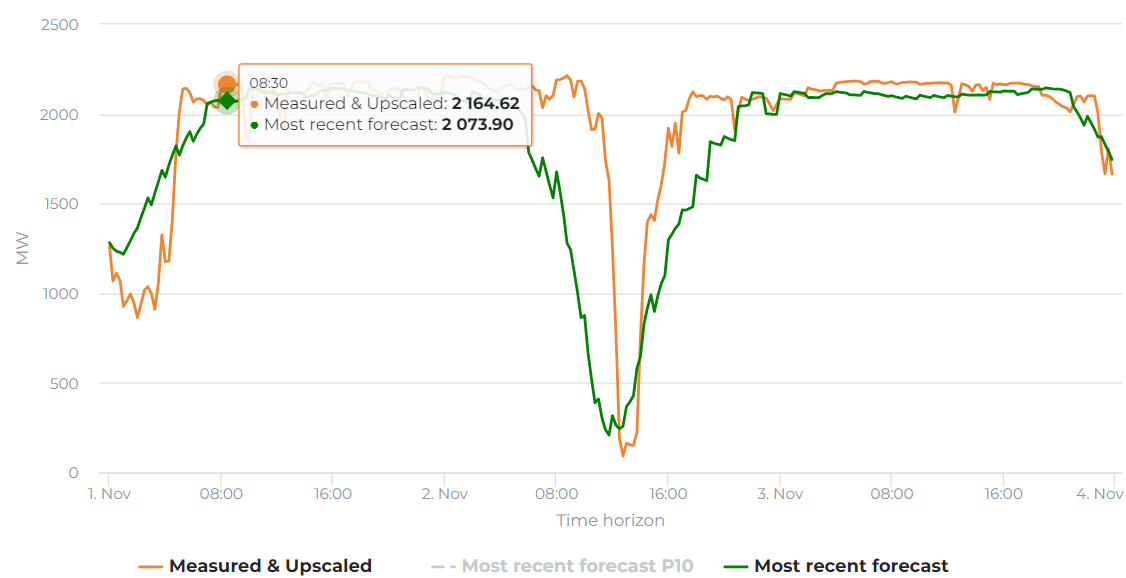
\includegraphics[width=\linewidth]{images/elia_storm_offshorewind_20231102.PNG}
    \end{center}
\end{column}
\end{columns}
\end{frame}

\begin{frame}{The Multi-Scale Frequency Control Hierarchy}
\footnotesize
Frequency restoration is coordinated across distinct physical and market layers:
\vspace{0.3cm}

\begin{center}
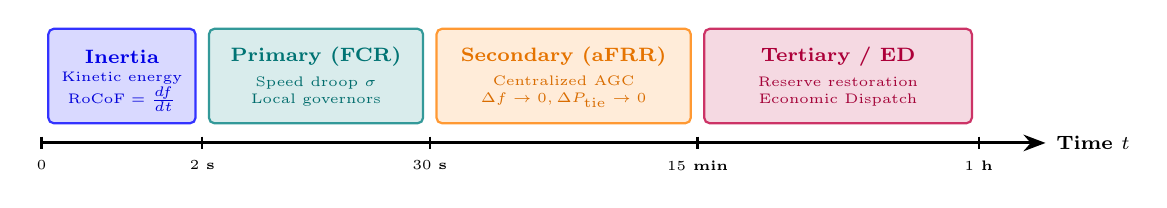
\begin{tikzpicture}[x=1.70cm, y=1.0cm, >=Stealth]
  % Timeline axis
  \draw[->, thick, line width=1.1pt] (0, 0) -- (7.5, 0) node[right, font=\scriptsize\bfseries] {Time $t$};
  
  % Ticks
  \foreach \x/\t in {0/{$0$}, 1.2/{$2\text{ s}$}, 2.9/{$30\text{ s}$}, 4.9/{$15\text{ min}$}, 7.0/{$1\text{ h}$}} {
    \draw[thick] (\x, 0.08) -- (\x, -0.08);
    \node[below, font=\tiny\bfseries] at (\x, -0.1) {\t};
  }
  
  % Stage 0: Inertia
  \draw[fill=blue!15, draw=blue!80, thick, rounded corners=2pt] (0.05, 0.25) rectangle (1.15, 1.45);
  \node[font=\scriptsize\bfseries, text=blue!90!black] at (0.6, 1.1) {Inertia};
  \node[font=\tiny, align=center, text=blue!85!black] at (0.6, 0.65) {Kinetic energy\\$\mathrm{RoCoF} = \frac{df}{dt}$};
  
  % Stage 1: Primary (FCR)
  \draw[fill=teal!15, draw=teal!80, thick, rounded corners=2pt] (1.25, 0.25) rectangle (2.85, 1.45);
  \node[font=\scriptsize\bfseries, text=teal!90!black] at (2.05, 1.1) {Primary (FCR)};
  \node[font=\tiny, align=center, text=teal!85!black] at (2.05, 0.65) {Speed droop $\sigma$\\Local governors};
  
  % Stage 2: Secondary (aFRR / AGC)
  \draw[fill=orange!15, draw=orange!80, thick, rounded corners=2pt] (2.95, 0.25) rectangle (4.85, 1.45);
  \node[font=\scriptsize\bfseries, text=orange!90!black] at (3.9, 1.1) {Secondary (aFRR)};
  \node[font=\tiny, align=center, text=orange!85!black] at (3.9, 0.65) {Centralized AGC\\$\Delta f \to 0, \Delta P_{\text{tie}} \to 0$};
  
  % Stage 3: Tertiary (mFRR / ED)
  \draw[fill=purple!15, draw=purple!80, thick, rounded corners=2pt] (4.95, 0.25) rectangle (6.95, 1.45);
  \node[font=\scriptsize\bfseries, text=purple!90!black] at (5.95, 1.1) {Tertiary / ED};
  \node[font=\tiny, align=center, text=purple!85!black] at (5.95, 0.65) {Reserve restoration\\Economic Dispatch};
\end{tikzpicture}
\end{center}
\end{frame}

\begin{frame}{Frequency Dynamic Signature: The Frequency Nadir}
\begin{columns}[T]
\begin{column}{0.5\textwidth}
    \footnotesize
    \textbf{Dynamic Stages Following a Generation Loss ($\Delta P_L$):}
    \begin{enumerate}\setlength{\itemsep}{2pt}
        \item \textbf{Inertial Response ($0 - 2\text{ s}$):}
        Stored kinetic energy buffers the shortfall; initial deceleration is governed by the \textbf{Rate of Change of Frequency (RoCoF)}.
        \item \textbf{Frequency Nadir ($f_{\text{nadir}}$ at $2 - 6\text{ s}$):}
        Point where governor mechanical ramp equals the power deficit ($df/dt = 0$).
        \item \textbf{Primary Settling ($10 - 30\text{ s}$):}
        Quasi-steady state stabilized at $f_{\text{ss}} < f_N$ by droop.
        \item \textbf{Secondary Recovery ($1 - 15\text{ min}$):}
        AGC integral action drives frequency back to $50.0\text{ Hz}$ (not shown).
    \end{enumerate}
\end{column}
\begin{column}{0.48\textwidth}
    \begin{center}
    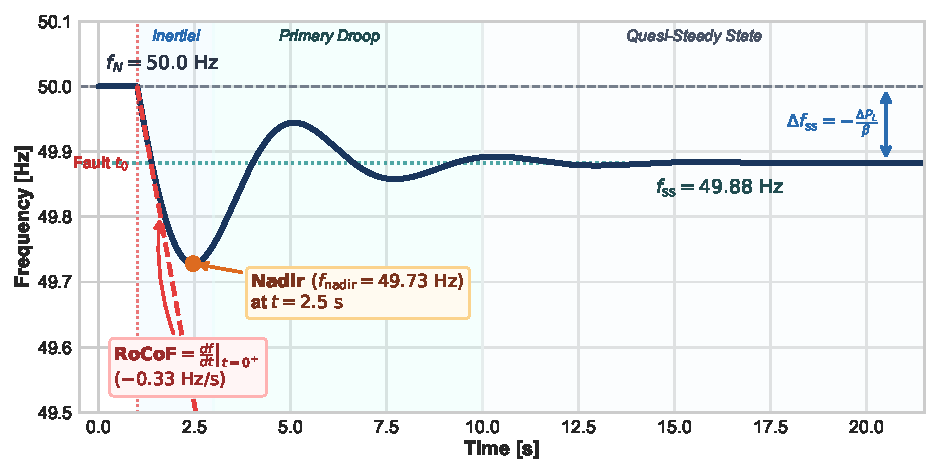
\includegraphics[width=\linewidth]{images/frequency_nadir.pdf}
    \end{center}
\end{column}
\end{columns}
\end{frame}

\begin{frame}{Control Resources: Levers for Frequency Stability}
\begin{columns}[T]
\begin{column}{0.65\textwidth}
    \textbf{Which resources directly act on frequency?}
    \begin{itemize}\setlength{\itemsep}{2pt}
        \item \alert{\textbf{Synchronous generator mechanical power:}} Main lever (valves/gates in thermal, gas, hydro units).
        \item \alert{\textbf{Battery Energy Storage Systems (BESS):}} Ultra-fast synthetic inertia and FCR (response within $< 200\text{ ms}$).
        \item \alert{\textbf{Fast start-up peakers (OCGT, hydro pumps):}} Secondary / tertiary replenishment.
        \item \alert{\textbf{Inverter curtailment / over-frequency control:}} Rapid downward regulation for solar PV and wind.
        \item \alert{\textbf{Demand-side response \& UFLS:}} Controlled load disconnection in emergency states.
    \end{itemize}
\end{column}
\begin{column}{0.35\textwidth}
    \begin{block}{Non-Frequency Levers}
    \scriptsize
    Field excitation ($E_f$), transformer taps (OLTC), and shunt capacitors control \textbf{voltage ($Q-V$)}, not frequency!
    \end{block}
\end{column}
\end{columns}
\end{frame}

\begin{frame}{System Frequency Evolution: Theory, Example, and Intuition}
\begin{columns}[T]
\begin{column}{0.65\textwidth}
    \footnotesize
    Before exploring multi-level frequency control, let us build intuition from a simplified physical power system model.
    \vspace{0.1cm}
    
    Consider an interconnected grid with loads and synchronous generators:
    \begin{itemize}\setlength{\itemsep}{2pt}
        \item $p_e(t)$ is the total electrical power absorbed by loads (including network transmission losses and generator conversion losses).
        \begin{itemize}
            \item By Kirchhoff's laws, this is the exact total active power generators must inject at every instant!
        \end{itemize}
        \item $p_m(t)$ is the total mechanical power delivered to generator turbine shafts.
    \end{itemize}
    \vspace{0.1cm}
    \alert{Fundamental Question:} \textbf{How does system frequency $f(t)$ (and rotor mechanical speed) evolve over time?}
\end{column}
\begin{column}{0.35\textwidth}
    \begin{block}{Physical Intuition}
    \scriptsize
    Electrical demand $p_e(t)$ is dictated by consumers. Mechanical power $p_m(t)$ is controlled by turbine valves. Any instantaneous imbalance accelerates or decelerates generator rotors!
    \end{block}
\end{column}
\end{columns}
\end{frame}

\begin{frame}{The Swing Equation}
\begin{columns}[T]
\begin{column}{0.65\textwidth}
    \footnotesize
    Consider a synchronous area operating near nominal frequency $f_N$. Group all synchronous machines into a single equivalent rotor with moment of inertia $J$.
    \vspace{0.15cm}
    
    Newton's second rotational law relates rotor acceleration $\alpha$ to torque:
    \begin{equation*}
        J \alpha = T_m - T_e
    \end{equation*}
    Since $p = T \omega$ and $\omega = 2\pi f$, we obtain:
    \begin{equation*}
        J \frac{df}{dt} = \frac{p_m - p_e}{4\pi^2 f}
    \end{equation*}
    Adding generator mechanical damping $D_g$ (friction, windage, damper windings):
    \begin{equation*}
        J \frac{df}{dt} = \frac{p_m - p_e}{4\pi^2 f} - {\color{myRed} D_g (f - f_N)}
    \end{equation*}
\end{column}
\begin{column}{0.35\textwidth}
    \begin{block}{Kinetic Buffer}
    \scriptsize
    When $p_e > p_m$, missing power is drawn directly from rotating kinetic energy $E_k = \frac{1}{2}J\omega^2$, causing $f(t)$ to decline.
    \end{block}
\end{column}
\end{columns}
\end{frame}

\begin{frame}{Inertia Constant of a Generator}
\begin{columns}[T]
\begin{column}{0.65\textwidth}
    \footnotesize
    The physical moment of inertia $J_i$ of generator $i$ is linked to its rated power $P_{\max,i}$ and dimensionless inertia constant $H_i$:
    \begin{equation*}
        J_i = \frac{2 P_{\max,i} H_i}{4 \pi^2 f_N^2} \quad [\text{kg}\cdot\text{m}^2]
    \end{equation*}
    where $f_N$ is nominal grid frequency ($50$ or $60\text{ Hz}$).
    \begin{itemize}\setlength{\itemsep}{2pt}
        \item $H_i$ (in seconds) represents the duration the machine can supply its rated power $P_{\max,i}$ solely from stored kinetic energy.
        \item Typical values: $H \approx 2 - 4\text{ s}$ for hydro, $H \approx 4 - 7\text{ s}$ for thermal units.
        \item In the swing equation, the total system inertia is $J = \sum_i J_i$.
    \end{itemize}
\end{column}
\begin{column}{0.35\textwidth}
    \begin{block}{System Inertia}
    \scriptsize
    In a coherent synchronous grid, all rotors swing in synchronism, acting as one giant equivalent flywheel of total inertia $J = \sum_i J_i$.
    \end{block}
\end{column}
\end{columns}
\end{frame}

\begin{frame}{What Happens If... (Interactive Questions)}
\begin{columns}[T]
\begin{column}{0.65\textwidth}
    \footnotesize
    \begin{block}{1. Power Imbalance (Sudden Load Increase $\Delta P_L$)?}
    \scriptsize
    Rotors immediately decelerate ($df/dt < 0$). Without governor intervention, frequency drops continuously until damping bounds it or the system collapses!
    \end{block}
    \begin{block}{2. Effect of Lower Inertia ($J \downarrow$)?}
    \scriptsize
    Steeper initial slope (higher $\mathrm{RoCoF} = |df/dt|$), leading to a faster and deeper frequency nadir.
    \end{block}
    \begin{block}{3. Effect of Damping ($D_g$)?}
    \scriptsize
    Provides natural resistive braking proportional to frequency deviation, moderating the decline.
    \end{block}
\end{column}
\begin{column}{0.35\textwidth}
    \begin{block}{Simulation Verification}
    \scriptsize
    Verify these 3 physical effects in the interactive notebook:
    \vspace{0.2cm}
    
    \href{https://github.com/bcornelusse/ELEC0447-analysis-power-systems/blob/master/Lectures/frequency_control/frequency_control_simulation.ipynb}{\beamergotobutton{Notebook: Cases 1--3}}
    \vspace{0.15cm}
    
    \tiny
    \begin{itemize}\setlength{\itemsep}{2pt}
        \item \textbf{Case 1:} No governor ($\sigma \to \infty$)
        \item \textbf{Case 2:} Low inertia ($J/10$)
        \item \textbf{Case 3:} Zero damping ($D_g = 0$)
    \end{itemize}
    \end{block}
\end{column}
\end{columns}
\end{frame}

\begin{frame}{Let's Add Generator Reaction to Frequency Change}
\begin{columns}[T]
\begin{column}{0.65\textwidth}
    \footnotesize
    \textbf{Why Inertia and Damping Are Not Enough:}
    \begin{itemize}\setlength{\itemsep}{3pt}
        \item Kinetic energy buffering is purely passive and temporary; it cannot restore power balance.
        \item Damping alone leaves an unacceptably large frequency deviation far below statutory limits ($\pm 200\text{ mHz}$).
        \item Therefore, generators must actively adjust their mechanical power output $p_m(t)$ in response to frequency changes!
    \end{itemize}
    \vspace{0.2cm}
    \textbf{The Primary Control Loop:}
    \begin{itemize}\setlength{\itemsep}{3pt}
        \item This fast automatic adjustment is \textbf{primary frequency control}.
        \item Let us analyze how a power plant's mechanical valve and speed governor are modeled.
    \end{itemize}
\end{column}
\begin{column}{0.35\textwidth}
    \begin{alertblock}{Control Necessity}
    \scriptsize
    To prevent continuous frequency decay, every major generator is equipped with a local speed governor.
    \end{alertblock}
\end{column}
\end{columns}
\end{frame}

\begin{frame}{Speed Governor of a Synchronous Generator}
\begin{columns}[T]
\begin{column}{0.55\textwidth}
  % 1. System Schematic (Governor in Green, Turbine in Red)
  \begin{center}
  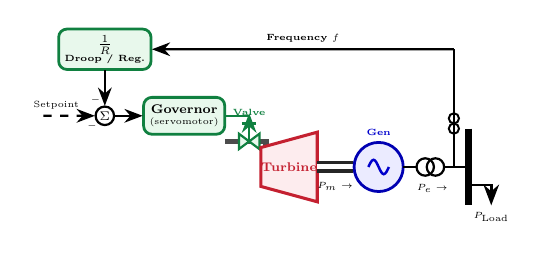
\begin{tikzpicture}[>=Stealth, font=\scriptsize, scale=0.65, transform shape]
    \definecolor{govGreen}{RGB}{16, 128, 64}
    \definecolor{govBg}{RGB}{232, 248, 236}
    \definecolor{turbRed}{RGB}{196, 32, 48}
    \definecolor{turbBg}{RGB}{253, 236, 238}

    % 1. Regulator block (Green)
    \node[draw=govGreen, fill=govBg, line width=1.0pt, rounded corners=3pt, minimum width=1.2cm, minimum height=0.75cm, align=center] 
      (reg) at (1.1, 2.3) {\small $\frac{1}{R}$\\[-1pt]\tiny\textbf{Droop / Reg.}};
      
    % 2. Summing junction
    \node[draw, circle, inner sep=1pt, line width=0.8pt] (sum) at (1.1, 1.0) {\scriptsize $\Sigma$};
    
    % Supplementary control input (dashed)
    \draw[->, thick, dashed] (-0.1, 1.0) -- (sum.west) 
      node[above, pos=0.25, font=\tiny, align=center] {Setpoint};
    \node[font=\tiny] at (0.85, 0.8) {$-$};
    \node[font=\tiny] at (0.92, 1.3) {$-$};
    
    % 3. Turbine governor / servomotor (Green)
    \node[draw=govGreen, fill=govBg, line width=1.0pt, rounded corners=3pt, minimum width=1.5cm, minimum height=0.72cm, align=center] 
      (gov) at (2.65, 1.0) {\scriptsize\textbf{Governor}\\[-2pt]\tiny(servomotor)};
      
    % 4. Valve & Pipe
    % Steam pipe
    \draw[line width=2.0pt, gray!60!black] (3.45, 0.5) -- (4.25, 0.5) -- (4.25, 0.35);
    % Valve symbol: two triangles meeting in the middle
    \filldraw[draw=govGreen, fill=govBg, line width=0.8pt] 
      (3.72, 0.65) -- (3.92, 0.5) -- (3.72, 0.35) -- cycle;
    \filldraw[draw=govGreen, fill=govBg, line width=0.8pt] 
      (4.12, 0.65) -- (3.92, 0.5) -- (4.12, 0.35) -- cycle;
    % Valve actuator stem & diaphragm
    \draw[line width=0.9pt, govGreen] (3.92, 0.5) -- (3.92, 0.85);
    \draw[line width=1.4pt, govGreen] (3.78, 0.85) -- (4.06, 0.85);
    \node[above=1pt, font=\tiny\bfseries, text=govGreen] at (3.92, 0.85) {Valve};
    
    % Connection governor -> valve
    \draw[->, line width=0.9pt, govGreen] (gov.east) -| (3.92, 1.05);
    
    % Connection regulator -> sum -> governor
    \draw[->, line width=0.8pt] (reg.south) -- (sum.north);
    \draw[->, line width=0.8pt] (sum.east) -- (gov.west);
    
    % 5. Turbine (Red trapezoid)
    \filldraw[draw=turbRed, fill=turbBg, line width=1.1pt] 
      (4.15, 0.38) -- (5.25, 0.68) -- (5.25, -0.68) -- (4.15, -0.38) -- cycle;
    \node[text=turbRed, font=\bfseries\scriptsize] at (4.7, 0.0) {Turbine};
    
    % 6. Shaft Turbine -> Generator
    \draw[line width=1.2pt, double, double distance=1.8pt, gray!30!black] (5.25, 0.0) -- (5.95, 0.0);
    \node[below, font=\tiny\bfseries] at (5.6, -0.18) {$P_m \rightarrow$};
    
    % 7. Generator (Circle)
    \filldraw[draw=blue!70!black, fill=blue!8, line width=1.0pt] (6.45, 0.0) circle (0.48cm);
    \draw[line width=0.9pt, blue!80!black] 
      (6.25, 0.0) sin (6.35, 0.14) cos (6.45, 0.0) sin (6.55, -0.14) cos (6.65, 0.0);
    \node[above, font=\tiny\bfseries, text=blue!80!black] at (6.45, 0.50) {Gen};
    
    % 8. Transformer & transmission line
    \draw[line width=0.8pt] (6.93, 0.0) -- (7.2, 0.0);
    % Transformer interlocking windings
    \draw[line width=0.8pt] (7.36, 0.0) circle (0.17cm);
    \draw[line width=0.8pt] (7.56, 0.0) circle (0.17cm);
    \draw[line width=0.8pt] (7.73, 0.0) -- (8.2, 0.0);
    \node[below, font=\tiny\bfseries] at (7.5, -0.22) {$P_e \rightarrow$};
    
    % 9. Busbar
    \draw[line width=2.4pt, black] (8.2, 0.75) -- (8.2, -0.75);
    % Load arrow
    \draw[->, line width=1.0pt] (8.2, -0.35) -- (8.65, -0.35) -- (8.65, -0.75) 
      node[below, font=\tiny\bfseries] {$P_{\mathrm{Load}}$};
    
    % 10. PT & Feedback loop
    \draw[line width=0.7pt] (7.92, 0.0) -- (7.92, 1.7);
    \draw[line width=0.7pt] (7.92, 0.75) circle (0.10cm);
    \draw[line width=0.7pt] (7.92, 0.95) circle (0.10cm);
    \draw[line width=0.7pt] (7.92, 1.7) -- (7.92, 2.3);
    \draw[->, line width=0.8pt] (7.92, 2.3) -- (reg.east) 
      node[above, midway, font=\tiny\bfseries] {Frequency $f$};
  \end{tikzpicture}
  \end{center}

  \vspace{-0.35cm}

  % 2. Steady-State Droop Characteristic Plot
  \begin{center}
  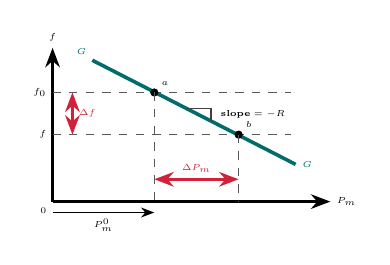
\begin{tikzpicture}[>=Stealth, font=\scriptsize, scale=0.63, transform shape]
    % Axes
    \draw[->, line width=0.9pt] (0, 0) -- (5.6, 0) node[right, font=\tiny\bfseries] {$P_m$};
    \draw[->, line width=0.9pt] (0, 0) -- (0, 3.1) node[above, font=\tiny\bfseries] {$f$};
    \node[below left, font=\tiny] at (0, 0) {$0$};
    
    % Reference dashed lines
    \draw[dashed, gray!70!black, line width=0.6pt] (0, 2.2) node[left, text=black, font=\tiny\bfseries] {$f_0$} -- (4.8, 2.2);
    \draw[dashed, gray!70!black, line width=0.6pt] (0, 1.35) node[left, text=black, font=\tiny\bfseries] {$f$} -- (4.8, 1.35);
    
    % Delta f indicator
    \draw[<->, line width=0.9pt, myRed] (0.4, 2.2) -- (0.4, 1.35) 
      node[midway, right, font=\tiny\bfseries] {$\Delta f$};
    
    % Droop line G-G
    \draw[line width=1.3pt, teal!85!black] (0.8, 2.85) -- (4.9, 0.75) 
      node[right, font=\tiny\bfseries] {$G$};
    \node[above left, font=\tiny\bfseries, text=teal!85!black] at (0.8, 2.85) {$G$};
    
    % Operating Points a and b
    \coordinate (A) at (2.05, 2.2);
    \coordinate (B) at (3.75, 1.35);
    
    \filldraw[black] (A) circle (2.0pt) node[above right=1pt, font=\tiny\bfseries] {$a$};
    \filldraw[black] (B) circle (2.0pt) node[above right=1pt, font=\tiny\bfseries] {$b$};
    
    % Dropping dashed lines
    \draw[dashed, gray!70!black, line width=0.5pt] (2.05, 2.2) -- (2.05, 0);
    \draw[dashed, gray!70!black, line width=0.5pt] (3.75, 1.35) -- (3.75, 0);
    
    % Delta Pm indicator
    \draw[<->, line width=0.9pt, myRed] (2.05, 0.45) -- (3.75, 0.45) 
      node[midway, above, font=\tiny\bfseries] {$\Delta P_m$};
    
    % Pm0 label
    \draw[->, thin] (0, -0.22) -- (2.05, -0.22) 
      node[midway, below, font=\tiny] {$P_m^0$};
    
    % Slope triangle
    \draw[line width=0.6pt, gray!50!black] (2.7, 1.88) -- (3.2, 1.88) -- (3.2, 1.63);
    \node[right=2pt, font=\tiny\bfseries, text=black] at (3.2, 1.76) {$\text{slope} = -R$};
  \end{tikzpicture}
  \end{center}
\end{column}
\begin{column}{0.42\textwidth}
    \scriptsize
    \begin{itemize}\setlength{\itemsep}{3pt}
        \item Rotor speed is continuously measured (or electrical frequency as a proxy).
        \item When frequency drops below $f_N$, the governor opens the valve to increase steam/gas/water mass flow.
        \item In steady state, frequency and mechanical power follow a \textbf{linear droop} characteristic.
        \item This relationship determines the generator's active power response during an imbalance.
        \item \textbf{Proportional control principle:} to trigger a power adjustment, frequency must deviate!
    \end{itemize}
\end{column}
\end{columns}
\end{frame}

\begin{frame}{Model of a Power Plant (Mechanical Part)}
\begin{columns}[T]
\begin{column}{0.55\textwidth}
    \begin{center}
    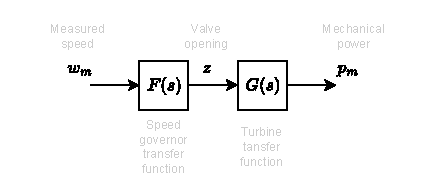
\includegraphics[width=\linewidth,height=4.8cm,keepaspectratio]{images/governor_and_turbine_transfer_function.pdf}
    \end{center}
\end{column}
\begin{column}{0.42\textwidth}
    \scriptsize
    \textbf{Mechanical Drive Components:}
    \begin{itemize}\setlength{\itemsep}{3pt}
        \item $\omega_m$ is the mechanical rotor speed (linked to electrical frequency $\omega$ by number of pole pairs).
        \item $z \in [0, 1]$ is the fractional opening of turbine control valves.
        \item $G(s)$ models the turbine response (converting valve opening $z$ into shaft torque/power $p_m$).
        \item We focus primarily on the \textbf{speed governor} block that commands $z$.
    \end{itemize}
\end{column}
\end{columns}
\end{frame}

\begin{frame}{Speed Governor Transfer Function}
\begin{columns}[T]
\begin{column}{0.58\textwidth}
    \begin{center}
    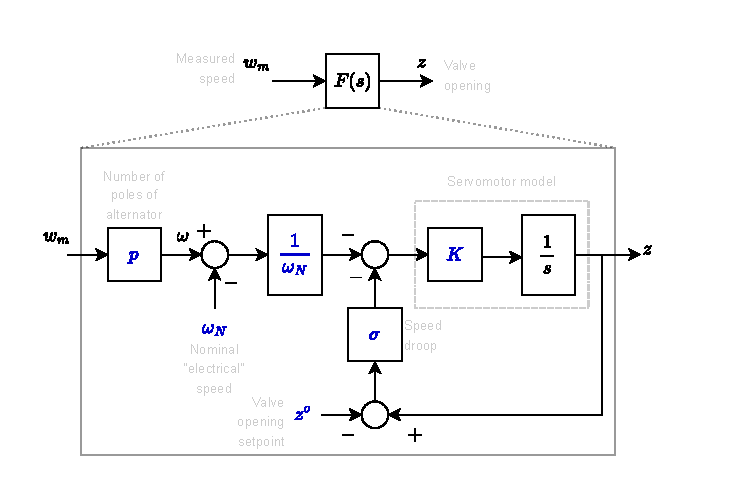
\includegraphics[width=\linewidth,height=4.8cm,keepaspectratio]{images/speed_governor_transfer_function.pdf}
    \end{center}
\end{column}
\begin{column}{0.39\textwidth}
    \scriptsize
    \textbf{Governor Signal Flow:}
    \begin{itemize}\setlength{\itemsep}{2pt}
        \item Rotor speed is scaled and compared to reference $\omega_N$ to generate a speed error signal.
        \item $z^o$ sets the desired power production setpoint at nominal frequency.
        \item In the feedback branch, valve position $z$ is compared to $z^o$ and scaled by droop $\sigma$.
        \item Net error drives the hydraulic servomotor (integrator with gain $K$) to adjust valve position $z$.
    \end{itemize}
\end{column}
\end{columns}
\end{frame}

\begin{frame}{Equivalent Block Diagram \& Governor Transfer Function}
\begin{columns}[T]
\begin{column}{0.55\textwidth}
    \begin{center}
    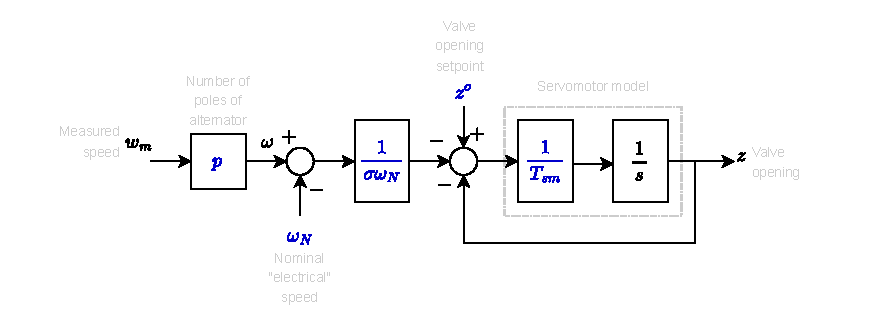
\includegraphics[width=\linewidth]{images/speed_governor_transfer_function_2.pdf}
    \end{center}
    \scriptsize
    \textbf{Servomotor Transfer Function:}
    \begin{itemize}\setlength{\itemsep}{2pt}
        \item Defining servomotor time constant $T_{sm} = \frac{1}{K \sigma}$ (typically $0.2 - 1.5\text{ s}$).
    \end{itemize}
\end{column}
\begin{column}{0.35\textwidth}
    \scriptsize    
    \begin{itemize}\setlength{\itemsep}{2pt}
        \item The closed-loop transfer function is:
        \begin{equation*}
            z(s) = \frac{1}{1 + s T_{sm}} \left( z^o - \frac{\omega - \omega_N}{\sigma \omega_N} \right)
        \end{equation*}
        \item In steady state ($s \to 0$):
        \begin{equation*}
            z = z^o - \frac{\omega - \omega_N}{\sigma \omega_N}
        \end{equation*}
    \end{itemize}
\end{column}
\end{columns}
\end{frame}

\begin{frame}{Steady-State Characteristic of a Turbine-Governor Set}
\begin{columns}[T]
\begin{column}{0.58\textwidth}
    \footnotesize
    In steady state ($s \to 0$):
    \begin{itemize}\setlength{\itemsep}{2pt}
        \item $p_m = G(0) z$ where $G(0)$ is the static turbine gain.
        \item At full valve opening ($z = 1$), turbine reaches nominal power $P_N = G(0) \cdot 1 \implies p_m = P_N z$.
        \item Substituting $z = z^o - \frac{\omega - \omega_N}{\sigma \omega_N}$:
        \begin{equation*}
            p_m = P_N z^o - \frac{P_N}{\sigma} \frac{f - f_N}{f_N}
        \end{equation*}
        \item Defining scheduled power setpoint $P^o = P_N z^o$:
        \begin{equation*}
            \boxed{p_m = P^o - \frac{P_N}{\sigma} \frac{f - f_N}{f_N}}
        \end{equation*}
        subject to physical limits $p_m \in [P_{\min}, P_{\max}]$.
    \end{itemize}
\end{column}
\begin{column}{0.40\textwidth}
    \centering
    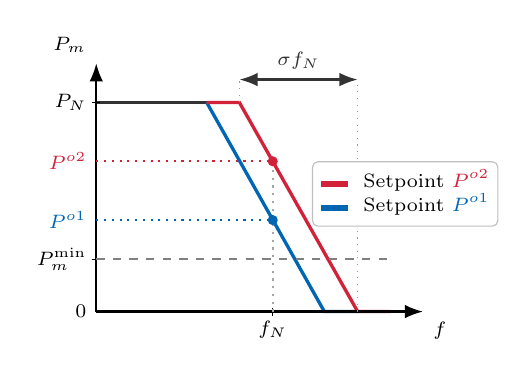
\begin{tikzpicture}[scale=0.83, >=Latex, font=\scriptsize]
        % Upper limit line at P_N
        \draw[thick, black!80] (0, 3.2) -- (1.69, 3.2);

        % Curve 1 (Blue, cPrimal): Setpoint P^{o1}
        \draw[very thick, cPrimal] (1.69, 3.2) -- (3.49, 0) -- (4.00, 0);

        % Curve 2 (Red, cDual): Setpoint P^{o2}
        \draw[very thick, cDual] (1.69, 3.2) -- (2.19, 3.2) -- (4.00, 0) -- (4.50, 0);

        % Coordinate Axes
        \draw[->, thick] (0,0) -- (5.0,0) node[below right] {$f$};
        \draw[->, thick] (0,0) -- (0,3.8) node[above left] {$P_m$};
        \node[left] at (0,0) {$0$};

        % Power limits on y-axis
        \node[left] at (0,3.2) {$P_N$};
        \draw (-0.06, 3.2) -- (0.06, 3.2);

        \node[left] at (0,0.8) {$P_m^{\min}$};
        \draw (-0.06, 0.8) -- (0.06, 0.8);
        \draw[dashed, black!50, thick] (0,0.8) -- (4.5,0.8);

        % Nominal frequency on x-axis
        \draw (2.7, -0.06) -- (2.7, 0.06);
        \node[below] at (2.7, 0) {$f_N$};

        % Vertical dotted line at f_N
        \draw[dotted, thick, gray!70] (2.7,0) -- (2.7,2.3);

        % Operating point 1 (cPrimal Blue)
        \draw[dotted, thick, cPrimal] (0,1.4) -- (2.7,1.4);
        \fill[cPrimal] (2.7,1.4) circle (2.2pt);
        \node[left, cPrimal, font=\bfseries\scriptsize] at (0,1.4) {$P^{o1}$};

        % Operating point 2 (cDual Red)
        \draw[dotted, thick, cDual] (0,2.3) -- (2.7,2.3);
        \fill[cDual] (2.7,2.3) circle (2.2pt);
        \node[left, cDual, font=\bfseries\scriptsize] at (0,2.3) {$P^{o2}$};

        % Droop width sigma f_N (span of Curve 2)
        \draw[dotted, gray!80] (2.19,3.2) -- (2.19,3.55);
        \draw[dotted, gray!80] (4.00,0) -- (4.00,3.55);
        \draw[<->, >=Latex, thick, black!80] (2.19,3.55) -- (4.00,3.55) node[midway, above] {$\sigma f_N$};

        % Legend
        \node[anchor=west, draw=black!25, fill=white, rounded corners=2pt, inner sep=3pt] at (3.3, 1.8) {
            \begin{tabular}{@{}l@{}}
                {\color{cDual}\rule{10pt}{2.2pt}} \ Setpoint ${\color{cDual}P^{o2}}$ \\
                {\color{cPrimal}\rule{10pt}{2.2pt}} \ Setpoint ${\color{cPrimal}P^{o1}}$
            \end{tabular}
        };
    \end{tikzpicture}
\end{column}
\end{columns}
\end{frame}

\begin{frame}{Time-Domain Turbine-Governor Model \& Limits}
\begin{columns}[T]
\begin{column}{0.65\textwidth}
    \footnotesize
    Transforming back to the time domain yields the first-order dynamic ODE for mechanical power:
    \begin{equation*}
        T_{sm} \frac{d p_m}{dt} = P^o - p_m - \frac{P_N}{\sigma} \frac{f - f_N}{f_N}
    \end{equation*}
    with typical parameters $T_{sm} \approx 0.5 - 2\text{ s}$ and droop $\sigma \approx 4\% - 6\%$.
    \vspace{0.15cm}
    
    \textbf{Physical Generator Boundaries:}
    \begin{equation*}
        p_m(t) \in [P_{\min}, P_{\max}]
    \end{equation*}
    \begin{itemize}\setlength{\itemsep}{2pt}
        \item If $p_m$ hits $P_{\max}$, upward reserve is exhausted (saturation).
        \item If $p_m$ hits $P_{\min}$, downward curtailment capability is lost.
    \end{itemize}
\end{column}
\begin{column}{0.35\textwidth}
    \begin{block}{Simulation Verification}
    \scriptsize
    Explore droop variations and saturation limits in the notebook:
    \vspace{0.2cm}
    
    \href{https://github.com/bcornelusse/ELEC0447-analysis-power-systems/blob/master/Lectures/frequency_control/frequency_control_simulation.ipynb}{\beamergotobutton{Notebook: Cases 4--7}}
    \vspace{0.15cm}
    
    \tiny
    \begin{itemize}\setlength{\itemsep}{1pt}
        \item \textbf{Case 4:} Standard 4\% droop
        \item \textbf{Case 5:} Lighter 8\% droop
        \item \textbf{Case 6:} Saturation at $P_{\max}$
        \item \textbf{Case 7:} Downward limit $P_{\min}$
    \end{itemize}
    \end{block}
\end{column}
\end{columns}
\end{frame}

\begin{frame}{About the Speed Droop $\sigma$ (Le Statisme)}
\begin{columns}[T]
\begin{column}{0.65\textwidth}
    \footnotesize
    \begin{block}{Speed Droop $\sigma$ Definition}
    \scriptsize
    The speed droop is the ratio between relative frequency deviation and relative power deviation:
    \begin{equation*}
        \sigma = \left| \frac{\Delta f / f_N}{\Delta P_m / P_N} \right| = \left| \frac{\Delta \omega / \omega_N}{\Delta P_m / P_N} \right|
    \end{equation*}
    \end{block}
    \begin{itemize}\setlength{\itemsep}{2pt}
        \item A frequency drop $\Delta f = \sigma f_N = 0.04 \times 50 = 2\text{ Hz}$ mobilizes $100\%$ nominal capacity ($\Delta P_m = P_N$).
        \item For normal primary activation band $\Delta f = -200\text{ mHz}$ ($-0.4\%$), a $4\%$ droop mobilizes $\frac{0.004}{0.04} P_N = 10\% P_N$.
        \item If $\sigma \to \infty$, the generator operates at constant power and does not participate in frequency control.
    \end{itemize}
\end{column}
\begin{column}{0.35\textwidth}
    \begin{alertblock}{Proportional Action}
    \scriptsize
    Because speed droop is a proportional controller:
    \begin{itemize}\setlength{\itemsep}{1pt}
        \item It inherently leaves a \textbf{steady-state error} ($\Delta f \neq 0$).
        \item But this error is the \textbf{common signal} that allows multiple plants to share the effort without communicating!
    \end{itemize}
    \end{alertblock}
\end{column}
\end{columns}
\end{frame}

\begin{frame}{The Power Consumed by the Load Is Frequency Dependent}
\begin{columns}[T]
\begin{column}{0.65\textwidth}
    \footnotesize
    In reality, load power demand varies with grid frequency:
    \begin{equation*}
        p_e(f) = P_e^o \left( 1 + D_l (f - f_N) \right)
    \end{equation*}
    where $P_e^o$ is nominal consumption, and $D_l \approx 1\% - 2\%$ per Hz ($0.01 - 0.02\text{ Hz}^{-1}$) is the load frequency sensitivity.
    \vspace{0.1cm}
    
    \textbf{Physical Origin:}
    \begin{itemize}\setlength{\itemsep}{1pt}
        \item Induction motors driving fans, pumps, and compressors slow down as frequency falls, drawing less mechanical power.
        \item Resistive loads (heaters, lighting) remain frequency-independent.
        \item Natural self-regulation provides an inherent stabilizing damping effect!
    \end{itemize}
\end{column}
\begin{column}{0.35\textwidth}
    \begin{block}{Stabilizing Feedback}
    \scriptsize
    When frequency drops, total load automatically decreases, reducing the active power deficit!
    \end{block}
\end{column}
\end{columns}
\end{frame}

\begin{frame}{The Impact of Renewable Generation}
\begin{columns}[T]
\begin{column}{0.65\textwidth}
    \footnotesize
    Assume non-synchronous renewable generation $p_{PV}(t)$ is added to the system.
    \vspace{0.05cm}
    
    \textbf{Which equation does it impact?}
    \begin{equation*}
        J \frac{df}{dt} = \frac{p_m - p_e + {\color{myRed} p_{PV}}}{4\pi^2 f} - D_g (f - f_N)
    \end{equation*}
    \textbf{Coupled Physical Model Summary:}
    \begin{align*}
        T_{sm} \frac{d p_m}{dt} &= P^o - p_m - \frac{P_N}{\sigma}\frac{f - f_N}{f_N}, \quad p_m \in [P_{\min}, P_{\max}] \\
        p_e &= P_e^o \left( 1 + D_l (f - f_N) \right)
    \end{align*}
    \textbf{Consequence of RES Growth:}
    \begin{itemize}\setlength{\itemsep}{1pt}
        \item When PV displaces synchronous generators, total inertia $J$ drops.
        \item An unexpected solar surge without control causes overfrequency.
    \end{itemize}
\end{column}
\begin{column}{0.35\textwidth}
    \begin{block}{Simulation Verification}
    \scriptsize
    Simulate a sudden $+30\text{ MW}$ solar surge without curtailment in the notebook:
    \vspace{0.2cm}
    
    \href{https://github.com/bcornelusse/ELEC0447-analysis-power-systems/blob/master/Lectures/frequency_control/frequency_control_simulation.ipynb}{\beamergotobutton{Notebook: Case 8}}
    \end{block}
\end{column}
\end{columns}
\end{frame}

\begin{frame}{PV Inverter Modeling \& Overfrequency Curtailment (LFSM-O)}
\begin{columns}[T]
\begin{column}{0.55\textwidth}
    \centering
    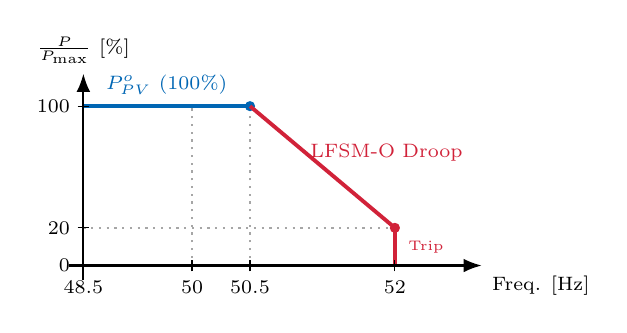
\begin{tikzpicture}[scale=0.92, >=Latex, font=\scriptsize]
        % Dotted base level at 0% up to 52 Hz
        \draw[dotted, thick, gray!60] (0.5, 0.3) -- (4.8, 0.3);

        % Dotted grid/projections
        \draw[dotted, thick, gray!70] (2.0, 0.3) -- (2.0, 2.50);
        \draw[dotted, thick, gray!70] (2.8, 0.3) -- (2.8, 2.50);
        \draw[dotted, thick, gray!70] (4.8, 0.3) -- (4.8, 0.82);
        \draw[dotted, thick, gray!70] (0.5, 0.82) -- (4.8, 0.82);

        % Profile Curve:
        % 1. Flat 100% (48.5 to 50.5 Hz)
        \draw[line width=1.4pt, cPrimal] (0.5, 2.50) -- (2.8, 2.50);
        \fill[cPrimal] (2.8, 2.50) circle (2pt);

        % 2. Droop Curtailment (50.5 to 52.0 Hz)
        \draw[line width=1.4pt, cDual] (2.8, 2.50) -- (4.8, 0.82);
        \fill[cDual] (4.8, 0.82) circle (2pt);

        % 3. Trip / Disconnection at 52 Hz
        \draw[line width=1.4pt, cDual] (4.8, 0.82) -- (4.8, 0.3);

        % 4. Zero injection after trip (f >= 52 Hz)
        \draw[line width=1.4pt, black!80] (4.8, 0.3) -- (5.6, 0.3);

        % Axes
        \draw[->, thick] (0.3, 0.3) -- (6.0, 0.3) node[below right, font=\scriptsize] {Freq. [Hz]};
        \draw[->, thick] (0.5, 0.1) -- (0.5, 2.95) node[above, font=\scriptsize, align=center] {$\frac{P}{P_{\max}}$ [\%]};

        % Y-axis ticks and labels
        \draw (0.42, 2.50) -- (0.58, 2.50);
        \node[left, font=\scriptsize] at (0.45, 2.50) {$100$};

        \draw (0.42, 0.82) -- (0.58, 0.82);
        \node[left, font=\scriptsize] at (0.45, 0.82) {$20$};

        \node[left, font=\scriptsize] at (0.45, 0.3) {$0$};

        % X-axis ticks and labels
        \draw (0.5, 0.22) -- (0.5, 0.38);
        \node[below, font=\scriptsize] at (0.5, 0.22) {$48.5$};

        \draw (2.0, 0.22) -- (2.0, 0.38);
        \node[below, font=\scriptsize] at (2.0, 0.22) {$50$};

        \draw (2.8, 0.22) -- (2.8, 0.38);
        \node[below, font=\scriptsize] at (2.8, 0.22) {$50.5$};

        \draw (4.8, 0.22) -- (4.8, 0.38);
        \node[below, font=\scriptsize] at (4.8, 0.22) {$52$};

        % Labels / Annotations
        \node[above, cPrimal, font=\scriptsize] at (1.65, 2.52) {$P_{PV}^o$ ($100\%$)};
        \node[above right, cDual, font=\scriptsize] at (3.5, 1.6) {LFSM-O Droop};
        \node[right, cDual, font=\tiny] at (4.85, 0.56) {Trip};
    \end{tikzpicture}
    \scriptsize
    \textbf{Piecewise Mathematical Model:}
    \begin{equation*}
        p_{PV}(f) = \begin{cases}
            P_{PV}^o & \text{if } f < 50.5\text{ Hz} \\
            P_{PV}^o \left[ 1 - \frac{0.8}{1.5}(f - 50.5) \right] & \text{if } 50.5 \le f < 52.0\text{ Hz} \\
            0 & \text{if } f \ge 52.0\text{ Hz}
        \end{cases}
    \end{equation*}
\end{column}
\begin{column}{0.42\textwidth}
    \scriptsize
    \textbf{Grid Code Mandates (ENTSO-E RfG):}
    \begin{itemize}\setlength{\itemsep}{2pt}
        \item Inverters cannot provide upward reserve unless pre-curtailed below MPPT.
        \item \textbf{LFSM-O (Overfrequency):} For $f \ge 50.2$ or $50.5\text{ Hz}$, active power must curtail automatically with a fast droop ($2\% - 12\%$).
        \item \textbf{LFSM-U (Underfrequency):} Pre-curtailed units ramp up power when $f < 49.8\text{ Hz}$.
    \end{itemize}
    \vspace{0.15cm}
    \href{https://github.com/bcornelusse/ELEC0447-analysis-power-systems/blob/master/Lectures/frequency_control/frequency_control_simulation.ipynb}{\beamergotobutton{Notebook: Cases 9 \& 10}}
\end{column}
\end{columns}
\end{frame}

%==============================================================================
% PART 2: Primary Frequency Control (Steady-State Multi-Machine Analysis)
%==============================================================================
\section{Primary Frequency Control}

\begin{frame}{Objective and Assumptions}
\begin{columns}[T]
\begin{column}{0.65\textwidth}
    \scriptsize
    Analyze the steady-state characteristics of primary control across an interconnected system under key assumptions:
    \begin{itemize}\setlength{\itemsep}{2pt}
        \item The post-disturbance system has settled to quasi-steady state ($10 - 30\text{ s}$).
        \item All synchronous machines rotate at the same electrical frequency ($f_1 = f_2 = \dots = f$).
        \item All participating generators are active within their operational bounds.
        \item Lossless transmission network ($\sum p_{mi} = p_e$).
        \item Mechanical turbine power is fully converted into electrical power.
        \item Load depends on frequency via sensitivity $D_l$: $p_e(f) = P_e^o(1 + D_l \Delta f)$.
        \item Initial operation is perfectly balanced at nominal frequency ($f = f_N$).
    \end{itemize}
\end{column}
\begin{column}{0.35\textwidth}
    \begin{block}{Core Question}
    \scriptsize
    How is a sudden load disturbance autonomously distributed among multiple participating plants without telecommunication?
    \end{block}
\end{column}
\end{columns}
\end{frame}

\begin{frame}{Parallel Operation: Two Generators Sharing a Load Increase}
\begin{columns}[T]
\begin{column}{0.5\textwidth} 
    \begin{center}
    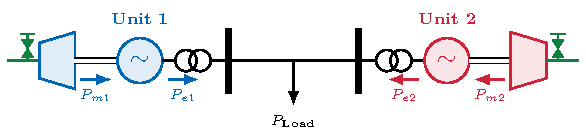
\includegraphics[width=\linewidth, height=2.3cm, keepaspectratio]{images/two_gen_schematic.pdf}        
    \end{center}
    \scriptsize
    \textbf{Autonomous Load Sharing:}
    \begin{itemize}\setlength{\itemsep}{1.5pt}
        \item Load increase $\Delta P_L \implies$ rotors decelerate, frequency drops ($\Delta f < 0$).
        \item Both governors open valves autonomously along droop curves (no communication).
        \item At steady state, power balance is restored:
        \begin{equation*}
            \Delta P_{m1} + \Delta P_{m2} = \Delta P_L
        \end{equation*}
    \end{itemize}
\end{column}
\begin{column}{0.45\textwidth}
    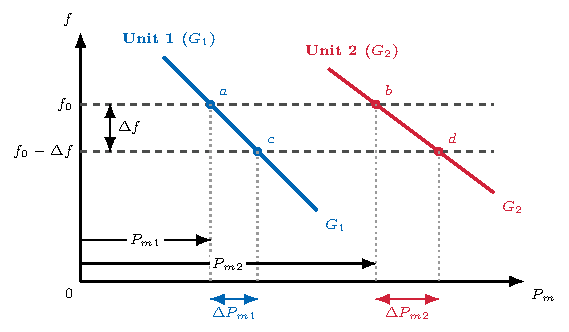
\includegraphics[width=\linewidth]{images/two_gen_primary_droop.pdf}
\end{column}
\end{columns}
\end{frame}

\begin{frame}{Share of Power Variation Among $n$ Generators}
\begin{columns}[T]
\begin{column}{0.65\textwidth}
    \scriptsize
    \setlength{\abovedisplayskip}{3pt}
    \setlength{\belowdisplayskip}{3pt}
    \textbf{Aggregating droop curves of $n$ machines} ($\Delta f = f - f_N$):
    \begin{equation*}
        p_m = \sum_{i=1}^n p_{mi} = \sum_{i=1}^n \left( P_i^o - \frac{\Delta f}{f_N} \frac{P_{Ni}}{\sigma_i} \right)
    \end{equation*}
    Power balance with demand disturbance $\Delta P_e$:
    \begin{equation*}
        \sum_{i=1}^n \left( P_i^o - \frac{\Delta f}{f_N} \frac{P_{Ni}}{\sigma_i} \right) = P_e^o (1 + D_l \Delta f) + {\color{myRed} \Delta P_e}
    \end{equation*}
    Using initial balance ($\sum P_i^o = P_e^o$) and rearranging:
    \begin{align*}
        -\frac{\Delta f}{f_N} \sum_{i=1}^n \frac{P_{Ni}}{\sigma_i} &= P_e^o D_l \Delta f + {\color{myRed} \Delta P_e} \\
        \implies \quad & \boxed{\Delta f = - \frac{\Delta P_e}{\beta}}
    \end{align*}
\end{column}
\begin{column}{0.35\textwidth}
    \begin{block}{Key Result}
    \scriptsize
    The steady-state frequency drop is directly proportional to the disturbance $\Delta P_e$ and inversely proportional to system stiffness $\beta$.
    \end{block}
\end{column}
\end{columns}
\end{frame}

\begin{frame}{System Stiffness ($\beta$) and Generator Participation}
\begin{columns}[T]
\begin{column}{0.60\textwidth}
    \footnotesize
    \begin{block}{Composite Frequency Response Characteristic ($\beta$)}
    \scriptsize
    \begin{equation*}
        \beta = \frac{1}{f_N} \sum_{i=1}^n \frac{P_{Ni}}{\sigma_i} + D_l P_e^o \quad [\text{MW/Hz}]
    \end{equation*}
    Also called \textit{network power frequency characteristic} or \textit{stiffness of system} (en français: \textit{énergie régulante}).
    \begin{itemize}\setlength{\itemsep}{1pt}
        \item Continental Europe: $\beta \approx 15\,000 - 25\,000\text{ MW/Hz}$ ($\approx 1500 - 2500\text{ MW}$ per $0.1\text{ Hz}$).
    \end{itemize}
    \end{block}
    
    \begin{block}{Variation of Power of $j$-th Generator}
    \scriptsize
    \begin{equation*}
        \Delta P_{mj} = - \frac{\Delta f}{f_N} \frac{P_{Nj}}{\sigma_j} = \boxed{\frac{\Delta P_e}{\beta} \frac{P_{Nj}}{\sigma_j f_N}}
    \end{equation*}
    \end{block}
\end{column}
\begin{column}{0.38\textwidth}
    \scriptsize
    \textbf{Load Sharing Properties:}
    \begin{itemize}\setlength{\itemsep}{2pt}
        \item \textbf{Size rule:} Larger rated power $P_{Nj} \implies$ larger contribution.
        \item \textbf{Droop rule:} Smaller droop $\sigma_j$ (steeper curve) $\implies$ larger contribution.
        \item \textbf{System scale:} More participating generators $\implies$ larger $\beta$, smaller $\Delta f$.
    \end{itemize}
\end{column}
\end{columns}
\end{frame}

\begin{frame}{Primary Reserve (FCR) Market Structure}
\begin{columns}[T]
\begin{column}{0.65\textwidth}
    \scriptsize
    \textbf{Operational Headroom \& Eligibility:}
    \begin{itemize}\setlength{\itemsep}{2pt}
        \item Only certified units participate in Frequency Containment Reserve (FCR).
        \item Generators must maintain headroom: $p_m \in [P_{\min} + R, P_{\max} - R]$.
        \item Base-load nuclear units rarely ramp; renewables offer mostly downward reserve.
    \end{itemize}
    \vspace{0.1cm}
    \textbf{ENTSO-E Regulatory Framework:}
    \begin{itemize}\setlength{\itemsep}{2pt}
        \item Reference incident sizing: $N-2 = 3000\text{ MW}$ in Continental Europe.
        \item Symmetrical full activation band: $\pm 200\text{ mHz}$ ($49.8 - 50.2\text{ Hz}$).
        \item Deployment within \textbf{30 seconds}; endurance $\ge 15\text{ minutes}$.
        \item Capacity procured through competitive regional market auctions.
    \end{itemize}
\end{column}
\begin{column}{0.35\textwidth}
    \begin{block}{End of Part 2}
    \scriptsize
    \textbf{Shortcomings of Primary Control:}
    \begin{enumerate}\setlength{\itemsep}{1pt}
        \item Residual error: $\Delta f \neq 0$.
        \item Unscheduled cross-border tie-line flows!
    \end{enumerate}
    $\implies$ Motivates Secondary Control (AGC)!
    \end{block}
\end{column}
\end{columns}
\end{frame}

%==============================================================================
% PART 3: Secondary Frequency Control (AGC / aFRR) (~20 min)
%==============================================================================
\section{Secondary Frequency Control (AGC / aFRR)}

%\begin{frame}{Secondary Frequency Control (AGC / aFRR)}
%\begin{columns}[T]
%\begin{column}{0.65\textwidth}
%    \footnotesize
%    \textbf{Recording Unit 3 ($\approx 20$ minutes):}
%    \begin{itemize}\setlength{\itemsep}{2pt}
%        \item The shortcomings of primary control: $\Delta f \neq 0$ and unscheduled transit.
%        \item Two interconnected control areas: mutual assistance vs contract deviations.
%        \item \textbf{Area Control Error (ACE):} Isolating the origin of disturbance.
%        \item Selection and tuning of the frequency bias factor $\lambda_i = \beta_i$.
%        \item Centralized PI controller architecture and participation factors $\rho_k$.
%        \item European balancing platforms: \textbf{PICASSO}.
%    \end{itemize}
%\end{column}
%\begin{column}{0.35\textwidth}
%    \begin{alertblock}{Key Objective}
%    \scriptsize
%    Understand how centralized secondary control coordinates multinational interconnections, drives $\Delta f \to 0$, and restores contract tie-line exchanges.
%    \end{alertblock}
%\end{column}
%\end{columns}
%\end{frame}

\begin{frame}{Why Do We Need Secondary Frequency Control?}
\begin{columns}[T]
\begin{column}{0.65\textwidth}
    \footnotesize
    Primary control achieves power balance, but leaves three critical shortcomings:
    \begin{enumerate}\setlength{\itemsep}{3pt}
        \item \textbf{Persistent Frequency Offset:} $\Delta f = -\Delta P_e / \beta \neq 0$. Clocks and synchronized equipment drift over time.
        \item \textbf{Unscheduled Cross-Border Flows:} Neighboring countries help absorb the imbalance, violating commercial tie-line contracts ($\Delta P_{\text{tie}} \neq 0$).
        \item \textbf{Depleted Primary Reserves:} Synchronous generators are left running away from nominal setpoints, leaving zero headroom for a second fault!
    \end{enumerate}
\end{column}
\begin{column}{0.35\textwidth}
    \begin{block}{Mission of AGC}
    \scriptsize
    Automatic Generation Control (AGC / aFRR) deploys within $0.5 - 15\text{ min}$ to drive both $\Delta f \to 0$ and $\Delta P_{\text{tie}} \to 0$, restoring primary reserves.
    \end{block}
\end{column}
\end{columns}
\end{frame}

\begin{frame}{Secondary Control: Governor Setpoint Adjustment}
\begin{columns}[T]
\begin{column}{0.58\textwidth}
    \centering
    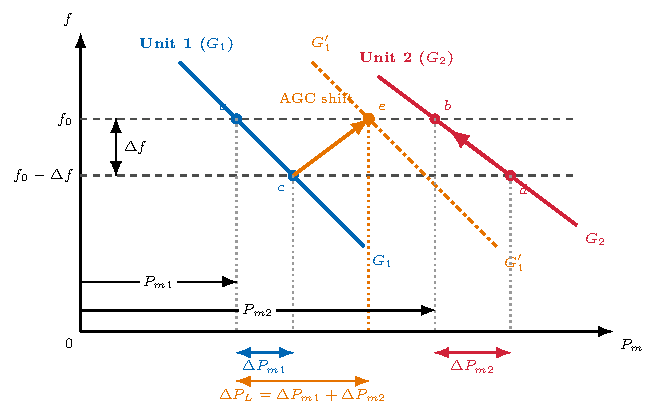
\includegraphics[width=\linewidth,height=4.8cm,keepaspectratio]{images/two_gen_secondary_droop.pdf}
\end{column}
\begin{column}{0.40\textwidth}
    \scriptsize
    \textbf{Secondary Action (AGC):}
    \begin{itemize}\setlength{\itemsep}{1.5pt}
        \item \textbf{Setpoint Shift:} AGC adjusts Unit 1 speed changer ($G_1 \to G_1'$).
        \item \textbf{Restoration:} Frequency returns to nominal ($f \to f_0$).
        \item \textbf{Reserve Recovery:} Unit 2 rides $G_2$ back to point $b$, fully recovering its primary reserve.
        \item \textbf{Result:} Unit 1 covers the entire load increase $\Delta P_L$ (point $e$).
    \end{itemize}
\end{column}
\end{columns}
\end{frame}

\begin{frame}{Two Interconnected Areas: Physical Model}
\begin{columns}[T]
\begin{column}{0.60\textwidth}
    \footnotesize
    Consider two synchronous areas interconnected by AC tie-lines:
    \begin{itemize}\setlength{\itemsep}{1pt}
        \item Area 1: $P_{m1} = P_{e1} + P_{12}$
        \item Area 2: $P_{m2} = P_{e2} - P_{12}$
    \end{itemize}
    where $P_{12}$ is the net export flow from Area 1 to Area 2.
    
    \textbf{Disturbance Scenario:}
    Sudden load increase $\Delta P_{e1}$ in Area 1.
    Primary droop responds across \textbf{both} areas:
    \begin{align*}
        -\beta_1 \Delta f &= \Delta P_{e1} + \Delta P_{12} \\
        -\beta_2 \Delta f &= -\Delta P_{12}
    \end{align*}
\end{column}
\begin{column}{0.40\textwidth}
    \begin{center}
    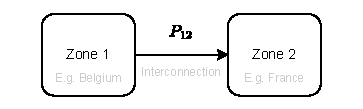
\includegraphics[width=\linewidth,height=3.0cm,keepaspectratio]{images/zones.pdf}
    \end{center}
\end{column}
\end{columns}
\end{frame}

\begin{frame}{Analysis of the Two-Area Interconnection}
\begin{columns}[T]
\begin{column}{0.65\textwidth}
    \footnotesize
    Summing the two equations yields total frequency deviation:
    \begin{equation*}
        \Delta f = - \frac{\Delta P_{e1}}{\beta_1 + \beta_2}
    \end{equation*}
    Substituting $\Delta f$ back into Area 2 equation gives tie-line flow deviation:
    \begin{equation*}
        \Delta P_{12} = - \frac{\beta_2}{\beta_1 + \beta_2} \Delta P_{e1} < 0
    \end{equation*}
    \begin{itemize}\setlength{\itemsep}{1pt}
        \item Power flows from Area 2 into Area 1 to support the deficit.
        \item Area 2 generators are supporting Area 1 at their own expense!
        \item Secondary control in Area 1 must increase internal production so Area 2 can return to its scheduled exchange $P_{12}^0$.
    \end{itemize}
\end{column}
\begin{column}{0.35\textwidth}
    \begin{block}{Responsibility Principle}
    \scriptsize
    The area where the imbalance originated must activate secondary reserve to bring its net interchange back to schedule!
    \end{block}
\end{column}
\end{columns}
\end{frame}

\begin{frame}{Exercise: Two-Area Primary Response}
\footnotesize
\textbf{System Data:}
Two interconnected synchronous areas:
\begin{itemize}\setlength{\itemsep}{1pt}
    \item Area 1: $\beta_1 = 10\,000\text{ MW/Hz}$, \quad Area 2: $\beta_2 = 15\,000\text{ MW/Hz}$
    \item Initial state: $f_0 = 50.000\text{ Hz}$, scheduled tie-line exchange $P_{12}^0 = 0\text{ MW}$
    \item Disturbance: sudden load step in Area 1 of ${\color{myRed}\Delta P_{e1} = +1\,000\text{ MW}}$ ($\Delta P_{e2} = 0$).
\end{itemize}

\vspace{2pt}
\textbf{Questions:}
\begin{enumerate}\setlength{\itemsep}{2pt}
    \item Compute the new quasi-steady-state frequency deviation $\Delta f$.
    \item Compute the primary power response ($\Delta P_{m1}, \Delta P_{m2}$) in each area.
    \item Determine the unscheduled tie-line power flow deviation $\Delta P_{12}$ ($1 \to 2$). Which area supports which?
\end{enumerate}

\vfill
% Room for handwritten solution
\end{frame}

\begin{frame}{Solution: Two-Area Primary Response}
\begin{columns}[T]
\begin{column}{0.62\textwidth}
    \scriptsize
    \textbf{System Data:}
    \begin{itemize}\setlength{\itemsep}{1pt}
        \item Area 1: $\beta_1 = 10\,000\text{ MW/Hz}$, \quad Area 2: $\beta_2 = 15\,000\text{ MW/Hz}$
        \item Disturbance: sudden load step in Area 1 of ${\color{myRed}\Delta P_{e1} = +1\,000\text{ MW}}$.
    \end{itemize}
    \vspace{1pt}
    \textbf{1. Frequency Deviation ($\Delta f$):}
    \begin{equation*}
        \setlength{\abovedisplayskip}{2pt}\setlength{\belowdisplayskip}{2pt}
        \Delta f = - \frac{\Delta P_{e1}}{\beta_1 + \beta_2} = - \frac{1\,000}{25\,000} = \mathbf{-0.040\text{ Hz}} \quad (-40\text{ mHz})
    \end{equation*}
    \textbf{2. Primary Response per Area ($\Delta P_{mi} = -\beta_i \Delta f$):}
    \begin{itemize}\setlength{\itemsep}{1pt}
        \item Area 1: $\Delta P_{m1} = -10\,000 \times (-0.04) = \mathbf{+400\text{ MW}}$ \quad (40\%)
        \item Area 2: $\Delta P_{m2} = -15\,000 \times (-0.04) = \mathbf{+600\text{ MW}}$ \quad (60\%)
    \end{itemize}
    \vspace{1pt}
    \textbf{3. Unscheduled Tie-Line Flow Deviation ($1 \to 2$):}
    \begin{equation*}
        \setlength{\abovedisplayskip}{2pt}\setlength{\belowdisplayskip}{2pt}
        \Delta P_{12} = \beta_2 \Delta f = 15\,000 \times (-0.04) = \mathbf{-600\text{ MW}}
    \end{equation*}
    $\implies$ \textbf{600 MW flows from Area 2 into Area 1} to help cover the deficit!
\end{column}
\begin{column}{0.36\textwidth}
    \begin{block}{Physical Interpretation}
    \scriptsize
    \begin{itemize}\setlength{\itemsep}{2pt}
        \item Area 2 automatically covers \textbf{60\%} of Area 1's deficit through local droop!
        \item Tie-line flow drops by $600\text{ MW}$, violating commercial exchange schedules.
        \item Area 2's primary reserves are depleted for Area 1's event.
    \end{itemize}
    \end{block}
\end{column}
\end{columns}
\end{frame}

\begin{frame}{The Area Control Error (ACE)}
\begin{columns}[T]
\begin{column}{0.65\textwidth}
    \footnotesize
    To localize the imbalance without inter-TSO real-time communication, each area $i$ computes its \textbf{Area Control Error (ACE)}:
    \begin{equation*}
        \text{ACE}_i = \Delta P_{\text{tie},i} + \lambda_i \Delta f
    \end{equation*}
    where:
    \begin{itemize}\setlength{\itemsep}{2pt}
        \item $\Delta P_{\text{tie},i} = P_{\text{tie},i} - P_{\text{tie},i}^0$ is net tie-line power flow deviation (export positive).
        \item $\Delta f = f - f_N$ is global frequency deviation.
        \item $\lambda_i > 0$ is the \textbf{frequency bias factor} $[\text{MW/Hz}]$.
    \end{itemize}
\end{column}
\begin{column}{0.35\textwidth}
    \begin{block}{Sign Convention}
    \scriptsize
    If $\text{ACE}_i < 0$, Area $i$ has an internal active power deficit and must increase generation.
    \end{block}
\end{column}
\end{columns}
\end{frame}

\begin{frame}{Exercise: Area Control Error (ACE)}
\footnotesize
\textbf{Context from previous primary response state:}
\begin{itemize}\setlength{\itemsep}{1pt}
    \item $\Delta f = -0.040\text{ Hz}$, \quad $\Delta P_{12} = -600\text{ MW}$ (net export $\Delta P_{\text{tie},1} = -600\text{ MW}$, $\Delta P_{\text{tie},2} = +600\text{ MW}$)
    \item Recall definition: $\text{ACE}_i = \Delta P_{\text{tie},i} + \lambda_i \Delta f$
\end{itemize}

\vspace{2pt}
\textbf{Questions:}
\begin{enumerate}\setlength{\itemsep}{2pt}
    \item Express $\text{ACE}_1(\lambda_1)$ and $\text{ACE}_2(\lambda_2)$ with frequency bias factors $\lambda_1, \lambda_2$ as parameters.
    \item What value must $\lambda_2$ take so that Area 2 (unaffected area) does not deploy secondary control ($\text{ACE}_2 = 0$)?
    \item If $\lambda_1 = \beta_1 = 10\,000\text{ MW/Hz}$, evaluate $\text{ACE}_1$. How does it relate to the initial disturbance $\Delta P_{e1}$?
\end{enumerate}

\vfill
% Room for handwritten solution
\end{frame}

\begin{frame}{Solution: Area Control Error (ACE)}
\begin{columns}[T]
\begin{column}{0.62\textwidth}
    \scriptsize
    \textbf{From the previous primary response state:}
    \begin{itemize}\setlength{\itemsep}{1pt}
        \item $\Delta f = -0.040\text{ Hz}$, \quad $\Delta P_{12} = -600\text{ MW}$ (Area 2 exports to Area 1)
        \item $\Delta P_{\text{tie},1} = \Delta P_{12} = -600\text{ MW}$, \quad $\Delta P_{\text{tie},2} = -\Delta P_{12} = +600\text{ MW}$
    \end{itemize}
    \vspace{2pt}
    \textbf{1. Expressing ACE with $\lambda$ as a parameter:}
    \begin{align*}
        \setlength{\abovedisplayskip}{2pt}\setlength{\belowdisplayskip}{2pt}
        \text{ACE}_1(\lambda_1) &= \Delta P_{\text{tie},1} + \lambda_1 \Delta f = \mathbf{-600 - 0.040\,\lambda_1} \\
        \text{ACE}_2(\lambda_2) &= \Delta P_{\text{tie},2} + \lambda_2 \Delta f = \mathbf{+600 - 0.040\,\lambda_2}
    \end{align*}
    \textbf{2. Condition for Area 2 (healthy) not to intervene ($\text{ACE}_2 = 0$):}
    \begin{equation*}
        \setlength{\abovedisplayskip}{2pt}\setlength{\belowdisplayskip}{2pt}
        600 - 0.040\,\lambda_2 = 0 \iff \lambda_2 = \frac{600}{0.040} = \mathbf{15\,000\text{ MW/Hz}} = \beta_2!
    \end{equation*}
    \textbf{3. Resulting ACE in Area 1 (with $\lambda_1 = \beta_1 = 10\,000\text{ MW/Hz}$):}
    \begin{equation*}
        \setlength{\abovedisplayskip}{2pt}\setlength{\belowdisplayskip}{2pt}
        \text{ACE}_1 = -600 - 0.040 \times 10\,000 = \mathbf{-1\,000\text{ MW}} = -\Delta P_{e1}
    \end{equation*}
    $\implies$ Area 1 AGC ramps up exactly $1\,000\text{ MW}$ of secondary reserves!
\end{column}
\begin{column}{0.36\textwidth}
    \begin{block}{Impact of Tuning $\lambda_2$}
    \scriptsize
    \begin{itemize}\setlength{\itemsep}{2pt}
        \item \textbf{Matched ($\lambda_2 = 15\,000$):}\\
        $\text{ACE}_2 = 0\text{ MW}$ $\implies$ zero secondary intervention.
        \item \textbf{Under-biased ($\lambda_2 = 10\,000$):}\\
        $\text{ACE}_2 = +200\text{ MW} > 0$ $\implies$ Area 2 backs off generation!
        \item \textbf{Over-biased ($\lambda_2 = 20\,000$):}\\
        $\text{ACE}_2 = -200\text{ MW} < 0$ $\implies$ Area 2 takes on Area 1's deficit!
    \end{itemize}
    \end{block}
\end{column}
\end{columns}
\end{frame}

\begin{frame}{Optimal Tuning of the Bias Factor $\lambda_i$}
\begin{columns}[T]
\begin{column}{0.65\textwidth}
    \footnotesize
    What happens if we choose $\lambda_2 = \beta_2$ for Area 2 (where no fault occurred)?
    \begin{align*}
        \text{ACE}_2 &= \Delta P_{\text{tie},2} + \lambda_2 \Delta f \\
                     &= - \Delta P_{12} + \beta_2 \left( - \frac{\Delta P_{e1}}{\beta_1 + \beta_2} \right) \\
                     &= - \left( - \frac{\beta_2}{\beta_1 + \beta_2}\Delta P_{e1} \right) - \frac{\beta_2}{\beta_1 + \beta_2}\Delta P_{e1} = 0!
    \end{align*}
    \begin{alertblock}{Fundamental Property of Tie-Line Bias Control}
    If each TSO tunes $\lambda_i = \beta_i$, \textbf{only the faulted area measures a non-zero ACE}! Healthy areas do not incorrectly react.
    \end{alertblock}
\end{column}
\begin{column}{0.35\textwidth}
    \begin{block}{Decentralized Intelligence}
    \scriptsize
    By matching $\lambda_i$ to stiffness $\beta_i$, multinational grids self-discriminate local vs external imbalances purely from local boundary flows!
    \end{block}
\end{column}
\end{columns}
\end{frame}

\begin{frame}{Centralized AGC Architecture}
\begin{columns}[T]
\begin{column}{0.60\textwidth}
    \footnotesize
    \textbf{Centralized Dispatch Loop at the TSO:}
    \begin{itemize}\setlength{\itemsep}{2pt}
        \item SCADA samples tie-line flows and grid frequency every $1 - 4\text{ s}$.
        \item ACE is fed into a Proportional-Integral (PI) controller:
        \begin{equation*}
            \Delta P_{\text{area}}^o = - K_p \text{ACE} - K_i \int \text{ACE} \, dt
        \end{equation*}
        \item In practice, $K_p \approx 0$ (pure integral control) to prevent fighting primary droop!
        \item When $\text{ACE} = 0 \implies \Delta f = 0$ and $\Delta P_{\text{tie}} = 0$.
    \end{itemize}
\end{column}
\begin{column}{0.40\textwidth}
    \begin{center}
    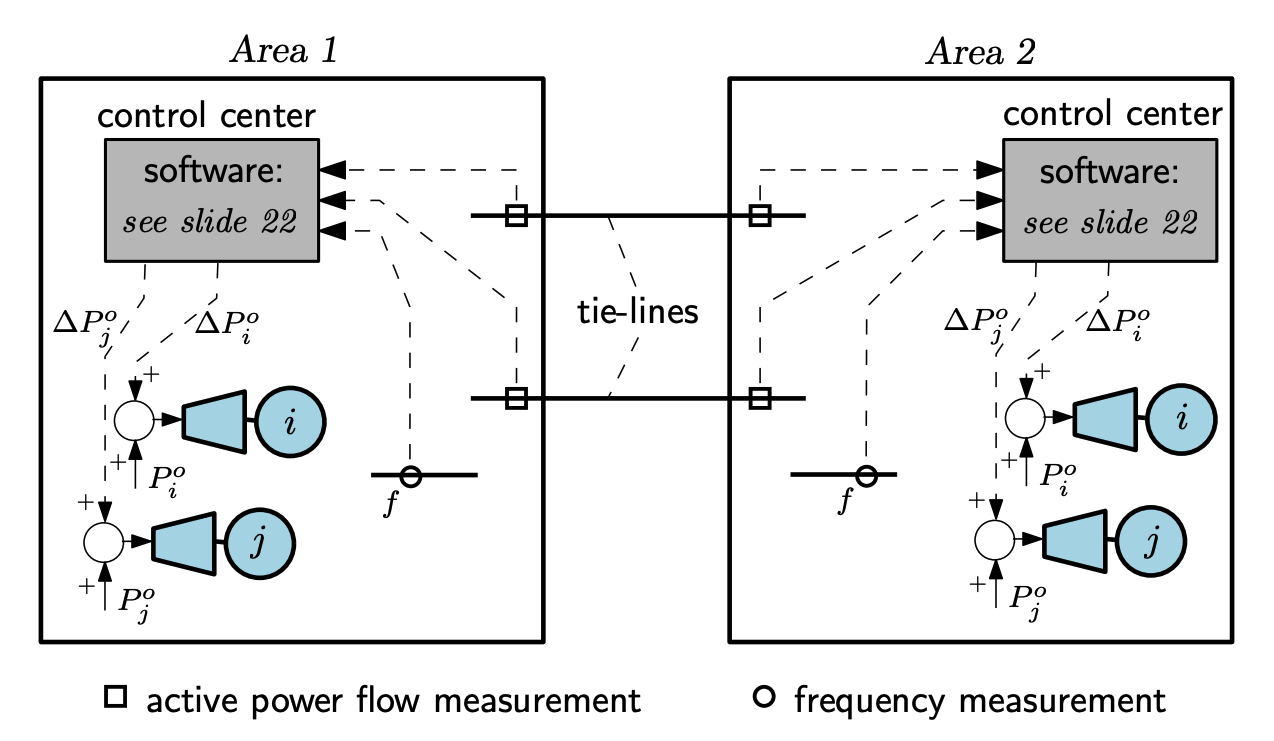
\includegraphics[width=\linewidth,height=3.2cm,keepaspectratio]{images/AGC_TWO_ZONES.png}
    \end{center}
\end{column}
\end{columns}
\end{frame}

\begin{frame}{Participation Factors \& Dynamic Ramp Constraints}
\begin{columns}[T]
\begin{column}{0.65\textwidth}
    \footnotesize
    The total area correction $\Delta P_{\text{area}}^o$ is distributed among contracted aFRR units:
    \begin{equation*}
        P_k^o \leftarrow P_k^o + \rho_k \Delta P_{\text{area}}^o \quad \text{with} \quad \sum_{k} \rho_k = 1
    \end{equation*}
    \begin{itemize}\setlength{\itemsep}{2pt}
        \item $\rho_k$: participation factor of generator $k$.
        \item \textbf{Unit ramp rates limits must be respected:}
        \begin{itemize}
            \item Hydro units: up to $100\% \, P_N / \text{min}$ (extremely agile).
            \item Thermal / CCGT units: $2\% - 6\% \, P_N / \text{min}$.
            \item Batteries: instantaneous response ($< 1\text{ s}$).
        \end{itemize}
        \item Anti-windup algorithms prevent integral saturation when units hit $P_{\max}$.
    \end{itemize}
\end{column}
\begin{column}{0.35\textwidth}
    \begin{block}{Setpoints vs Output}
    \scriptsize
    AGC adjusts governor \textbf{power setpoints} $P_k^o$, leaving the primary droop feedback loop fully intact to handle fast fluctuations!
    \end{block}
\end{column}
\end{columns}
\end{frame}

\begin{frame}{European Balancing Landscape: PICASSO}
\begin{columns}[T]
\begin{column}{0.65\textwidth}
    \footnotesize
    \textbf{The PICASSO Platform (ENTSO-E):}
    \begin{itemize}\setlength{\itemsep}{3pt}
        \item \textit{Platform for the International Coordination of Automated Frequency Restoration and Stable System Operation}.
        \item Optimizes the activation of aFRR bids across all participating European TSOs.
        \item Computes common merit-order activation every \textbf{4 seconds}.
        \item \textbf{Imbalance Netting:} If Belgium is short while Germany is long, their imbalances cancel out through cross-border capacity without activating expensive reserves!
    \end{itemize}
\end{column}
\begin{column}{0.35\textwidth}
    \begin{block}{End of Part 3}
    \scriptsize
    \textbf{Summary:} AGC restores frequency to $50\text{ Hz}$ and tie-lines to schedule. But who restores secondary reserve? \textbf{Tertiary control \& Economic Dispatch}!
    \end{block}
\end{column}
\end{columns}
\end{frame}

%==============================================================================
% PART 4: Tertiary Control, Economic Dispatch & OPF (~20 min)
%==============================================================================
\section{Tertiary Control, Economic Dispatch \& OPF}

%\begin{frame}{Tertiary Control, Economic Dispatch \& OPF}
%\begin{columns}[T]
%\begin{column}{0.65\textwidth}
%    \footnotesize
%    \textbf{Recording Unit 4 ($\approx 20$ minutes):}
%    \begin{itemize}\setlength{\itemsep}{2pt}
%        \item Role of tertiary control (mFRR \& Replacement Reserve).
%        \item \textbf{Economic Dispatch (ED):} Mathematical formulation.
%        \item Analytical solution: Lagrangian, KKT, and the Merit Order principle.
%        \item \textbf{Belgian Power System Case Study (ENVT3065):} Generation mix, dispatch dashboard, and merit order stack.
%        \item Why "copper plate" dispatch fails in real transmission grids.
%        \item \textbf{Optimal Power Flow (OPF):} Enforcing Kirchhoff's laws and grid security.
%    \end{itemize}
%\end{column}
%\begin{column}{0.35\textwidth}
%    \begin{alertblock}{Key Objective}
%    \scriptsize
%    Bridge system dynamics to economics and network physics: from merit order dispatch to security-constrained optimal power flow.
%    \end{alertblock}
%\end{column}
%\end{columns}
%\end{frame}

\begin{frame}{Tertiary Control: Manual Restoration (mFRR \& RR)}
\begin{columns}[T]
\begin{column}{0.65\textwidth}
    \footnotesize
    \textbf{Objectives of Tertiary Control ($15\text{ min} - 1\text{ h}$):}
    \begin{itemize}\setlength{\itemsep}{3pt}
        \item When a major outage persists, secondary reserves (aFRR) remain depleted.
        \item TSOs activate \textbf{Manual Frequency Restoration Reserve (mFRR)} via manual dispatch instructions.
        \item \textbf{Replacement Reserves (RR):} Start-up of slower thermal units or hydro pumped storage (e.g. Coo in Belgium) to relieve mFRR.
        \item \textbf{MARI platform:} Pan-European market for mFRR bid exchange.
        \item Once reserves are restored, unit operating setpoints are re-optimized via \textbf{Economic Dispatch}.
    \end{itemize}
\end{column}
\begin{column}{0.35\textwidth}
    \begin{block}{Time Scale}
    \scriptsize
    Tertiary control bridges real-time physical system balancing with intraday and day-ahead wholesale electricity markets!
    \end{block}
\end{column}
\end{columns}
\end{frame}

\begin{frame}{The Classical Economic Dispatch Problem}
\begin{columns}[T]
\begin{column}{0.65\textwidth}
    \footnotesize
    \textbf{Optimization Problem Statement:}
    Find active generation setpoints $\{\primal{P_i}\}_{i=1}^n$ that minimize total cost while meeting demand $P_L$:
    \begin{align*}
        \min_{\{\primal{P_i}\}} \quad & \sum_{i=1}^n C_i(\primal{P_i}) \\
        \text{s.t.} \quad & \sum_{i=1}^n \primal{P_i} = P_L + P_{\text{loss}} \quad \perp \quad \dual{\lambda} \\
                          & \underline{P}_i \le \primal{P_i} \le \overline{P}_i \quad \perp \quad \dual{\underline{\mu}_i, \overline{\mu}_i}, \quad \forall i=1,\dots,n
    \end{align*}
    where $C_i(\primal{P_i}) = a_i \primal{P_i}^2 + b_i \primal{P_i} + c_i$ is typically quadratic.
\end{column}
\begin{column}{0.35\textwidth}
    \begin{block}{Notation Convention}
    \scriptsize
    \begin{itemize}\setlength{\itemsep}{2pt}
        \item \primal{\textbf{Blue:}} Primal decision variables ($\primal{P_i}$).
        \item \dual{\textbf{Red:}} Dual variables / multipliers ($\dual{\lambda, \underline{\mu}_i, \overline{\mu}_i}$).
        \item \textbf{Black:} Fixed grid parameters ($P_L, \underline{P}_i, \overline{P}_i$).
        \item \textbf{$\perp$:} Complementarity / dual association with constraint.
    \end{itemize}
    \end{block}
\end{column}
\end{columns}
\end{frame}

\begin{frame}{Analytical Solution: Equal Incremental Cost Rule}
\begin{columns}[T]
\begin{column}{0.65\textwidth}
    \footnotesize
    Formulating the Lagrangian (neglecting losses for clarity):
    \begin{equation*}
        \mathcal{L}(\primal{P_i}, \dual{\lambda}) = \sum_{i=1}^n C_i(\primal{P_i}) - \dual{\lambda} \left( \sum_{i=1}^n \primal{P_i} - P_L \right)
    \end{equation*}
    First-order optimality condition ($\partial \mathcal{L}/\partial \primal{P_i} = 0$ for unconstrained units):
    \begin{equation*}
        \frac{dC_1}{d\primal{P_1}} = \frac{dC_2}{d\primal{P_2}} = \dots = \frac{dC_n}{d\primal{P_n}} = \dual{\lambda}
    \end{equation*}
    \begin{alertblock}{Merit Order Principle}
    All unconstrained generators must operate at the \textbf{exact same incremental marginal cost} $\dual{\lambda}$ [EUR/MWh], known as the \textbf{System Marginal Price (SMP)}!
    \end{alertblock}
\end{column}
\begin{column}{0.35\textwidth}
    \begin{block}{KKT Boundary Cases}
    \scriptsize
    \begin{itemize}\setlength{\itemsep}{2pt}
        \item If $dC_i/d\primal{P_i} > \dual{\lambda} \implies \primal{P_i} = \underline{P}_i \ (\dual{\underline{\mu}_i} > 0)$
        \item If $dC_i/d\primal{P_i} < \dual{\lambda} \implies \primal{P_i} = \overline{P}_i \ (\dual{\overline{\mu}_i} > 0)$
    \end{itemize}
    Units are stacked in ascending order of marginal cost!
    \end{block}
\end{column}
\end{columns}
\end{frame}

\begin{frame}{Case Study: Belgian Power System Generation Mix}
\begin{columns}[T]
\begin{column}{0.65\textwidth}
    \footnotesize
    \textbf{Structure of the Belgian Grid (ENVT3065):}
    \begin{itemize}\setlength{\itemsep}{2pt}
        \item Annual demand: $\approx 85\text{ TWh/year}$; peak load: $7 - 13\text{ GW}$.
        \item \textbf{Zero marginal cost:} Solar PV ($\sim 8\text{ GW}$ peak), Offshore wind ($2.3\text{ GW}$), Onshore wind ($\sim 3\text{ GW}$).
        \item \textbf{Baseload nuclear:} Doel 4 and Tihange 3 ($\sim 2\text{ GW}$ remaining post-extension, marginal cost $\approx 10-15\text{ EUR/MWh}$).
        \item \textbf{Mid-merit CCGT gas:} Combined Cycle Gas Turbines ($\sim 6\text{ GW}$, marginal cost $60 - 90\text{ EUR/MWh}$).
        \item \textbf{Peaking OCGT / Diesel:} Open cycle turbines ($> 150-250\text{ EUR/MWh}$).
        \item \textbf{Hydro Storage:} Coo-Trois-Ponts pumped hydro ($1.08\text{ GW}, 5.8\text{ GWh}$).
    \end{itemize}
\end{column}
\begin{column}{0.35\textwidth}
    \begin{block}{Belgian Merit Order}
    \scriptsize
    Renewables dispatch first $\to$ Nuclear baseload $\to$ CCGT gas $\to$ Peakers / imports set the marginal price $\dual{\lambda}$ in peak hours.
    \end{block}
\end{column}
\end{columns}
\end{frame}

\begin{frame}{Belgian Generation Dispatch in Action}
\begin{columns}[T]
\begin{column}{0.65\textwidth}
    \begin{center}
    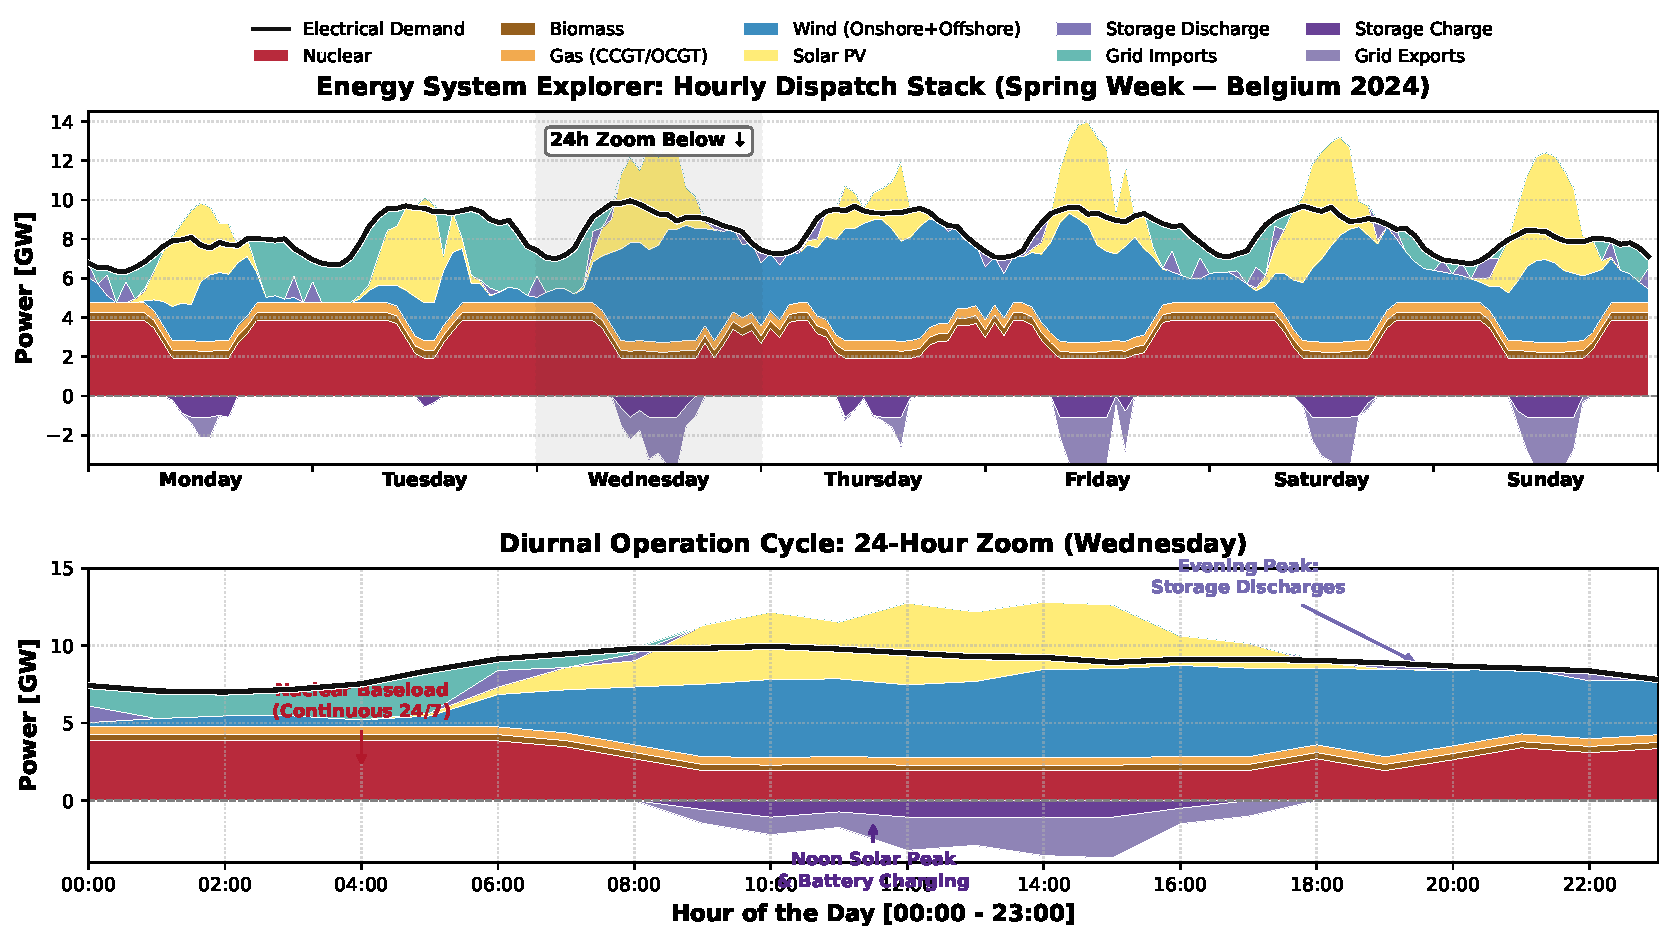
\includegraphics[width=\linewidth,height=5.6cm,keepaspectratio]{images/esx_dashboard_dispatch.pdf}
    \end{center}
\end{column}
\begin{column}{0.33\textwidth}
    \scriptsize
    \textbf{Operational Dynamics}
    \begin{itemize}\setlength{\itemsep}{2pt}
        \item \textbf{Top pane:} Generation stack (nuclear, CCGT, wind, solar).
        \item \textbf{Middle pane:} Coo pumped-storage cycling (pumping off-peak, generating on-peak).
        \item \textbf{Bottom pane:} Hourly System Marginal Price $\dual{\lambda}(t)$ [EUR/MWh].
        \item High RES output depresses $\dual{\lambda}$ towards zero (merit-order effect).
    \end{itemize}
\end{column}
\end{columns}
\end{frame}

\begin{frame}{Limitations of "Copper Plate" Economic Dispatch}
\begin{columns}[T]
\begin{column}{0.65\textwidth}
    \footnotesize
    \textbf{Why does Economic Dispatch fail in transmission grids?}
    \begin{itemize}\setlength{\itemsep}{2pt}
        \item Economic dispatch assumes power flows instantaneously and without impedance from any generator to any load.
        \item In reality, electrical power routes strictly according to \textbf{Kirchhoff's Laws} and branch impedances $\mathbf{Y}_{\text{bus}}$!
        \item Dispatching cheap northern offshore wind to supply southern industry can easily overload intermediate transmission corridors ($I_{ij} > I_{ij}^{\max}$).
        \item Voltage bounds ($0.95 \le V_k \le 1.05\text{ p.u.}$) and reactive power capabilities ($Q_{\min} \le Q_i \le Q_{\max}$) are completely ignored!
    \end{itemize}
\end{column}
\begin{column}{0.35\textwidth}
    \begin{alertblock}{Grid Congestion}
    \scriptsize
    When transmission lines saturate, TSOs must deviate from economic merit order: \textbf{preventive redispatch} or \textbf{Optimal Power Flow}!
    \end{alertblock}
\end{column}
\end{columns}
\end{frame}

\begin{frame}[allowframebreaks]{Optimal Power Flow (OPF): The Full Formulation}
\scriptsize
\textbf{The Full AC Optimal Power Flow (AC-OPF):}
\begin{align*}
    \min_{\primal{\mathbf{P}_G}, \primal{\mathbf{Q}_G}, \primal{\mathbf{V}}, \primal{\boldsymbol{\theta}}} \quad & \sum_{i \in \mathcal{G}} C_i(\primal{P_{Gi}}) \\
    \text{s.t.} \quad & \primal{P_{Gi}} - P_{Li} = \primal{V_i} \sum_{j \in \mathcal{N}} \primal{V_j} (G_{ij}\cos\primal{\theta_{ij}} + B_{ij}\sin\primal{\theta_{ij}}) \quad \perp \quad \dual{\lambda_{P,i}}, \quad \forall i \in \mathcal{N} \\
                      & \primal{Q_{Gi}} - Q_{Li} = \primal{V_i} \sum_{j \in \mathcal{N}} \primal{V_j} (G_{ij}\sin\primal{\theta_{ij}} - B_{ij}\cos\primal{\theta_{ij}}) \quad \perp \quad \dual{\lambda_{Q,i}}, \quad \forall i \in \mathcal{N} \\
                      & \underline{P}_{Gi} \le \primal{P_{Gi}} \le \overline{P}_{Gi} \quad \perp \quad \dual{\underline{\mu}_{P,i}, \overline{\mu}_{P,i}}, \quad \forall i \in \mathcal{G} \\
                      & \underline{Q}_{Gi} \le \primal{Q_{Gi}} \le \overline{Q}_{Gi} \quad \perp \quad \dual{\underline{\mu}_{Q,i}, \overline{\mu}_{Q,i}}, \quad \forall i \in \mathcal{G} \\
                      & V_i^{\min} \le \primal{V_i} \le V_i^{\max} \quad \perp \quad \dual{\underline{\mu}_{V,i}, \overline{\mu}_{V,i}}, \quad \forall i \in \mathcal{N} \\
                      & |S_{ij}(\primal{\mathbf{V}}, \primal{\boldsymbol{\theta}})| \le S_{ij}^{\max} \quad \perp \quad \dual{\mu_{S,ij}}, \quad \forall (i,j) \in \mathcal{L}
\end{align*}

\framebreak

\footnotesize
\textbf{Key Insights into OPF:}
\begin{itemize}\setlength{\itemsep}{3pt}
    \item \textbf{Mathematical Nature:} Large-scale, non-convex, non-linear optimization program.
    \item \textbf{DC-OPF Approximation:} For fast clearing, assume $\primal{V_i} \approx 1\text{ p.u.}$, line resistances $R \ll X$, and small angle differences ($\sin\primal{\theta_{ij}} \approx \primal{\theta_i} - \primal{\theta_j}$):
    \begin{equation*}
        \min_{\primal{\mathbf{P}_G}, \primal{\boldsymbol{\theta}}} \sum_{i \in \mathcal{G}} C_i(\primal{P_{Gi}}) \quad \text{s.t.} \quad \primal{\mathbf{P}_G} - \mathbf{P}_L = \mathbf{B}\primal{\boldsymbol{\theta}} \ \perp \ \dual{\boldsymbol{\lambda}}, \quad |B_{ij}(\primal{\theta_i} - \primal{\theta_j})| \le P_{ij}^{\max} \ \perp \ \dual{\mu_{ij}}
    \end{equation*}
    Solvable as a convex Quadratic or Linear Program (QP / LP)!
    \item \textbf{Locational Marginal Prices (LMP):} The dual variables $\dual{\lambda_i}$ at each bus reveal local nodal prices reflecting energy cost + transmission congestion losses.
\end{itemize}
\end{frame}

\begin{frame}{Synthesis: The Full Frequency Hierarchy}
\begin{center}
\scriptsize
\setlength{\tabcolsep}{4pt}
\renewcommand{\arraystretch}{1.15}
\resizebox{0.95\textwidth}{!}{%
\begin{tabular}{lllll}
\toprule
\textbf{Layer} & \textbf{Time Scale} & \textbf{Actuator} & \textbf{Objective} & \textbf{Market / Control} \\
\midrule
\textbf{Inertia} & $0 - 2\text{ s}$ & Synchronous rotors & Limit RoCoF ($df/dt$) & Physical / Grid-forming \\
\textbf{Primary (FCR)} & $2 - 30\text{ s}$ & Speed governors & Arrest nadir / $f_{\text{ss}}$ & Decentralized droop ($\sigma$) \\
\textbf{Secondary (aFRR)} & $0.5 - 15\text{ min}$ & Centralized AGC & $\Delta f \to 0, \Delta P_{\text{tie}} \to 0$ & PICASSO / PI loop \\
\textbf{Tertiary (mFRR)} & $15 - 60\text{ min}$ & Peakers, pumps & Restore aFRR & MARI / Manual dispatch \\
\textbf{Economic Dispatch} & $15\text{ min} - 1\text{ d}$ & Fleet scheduling & Minimize $\sum C_i$ & Merit Order / OPF \\
\bottomrule
\end{tabular}%
}
\end{center}
\end{frame}

\begin{frame}{Conclusion of Lecture}
\begin{columns}[T]
\begin{column}{0.65\textwidth}
    \footnotesize
    \textbf{Core Takeaways:}
    \begin{itemize}\setlength{\itemsep}{3pt}
        \item Frequency is a global system variable dictated by active power balance.
        \item Kinetic energy buffers initial shocks; droop controls arrest the fall.
        \item AGC restores nominal frequency and contracted exchanges without inter-TSO voice calls.
        \item Economic dispatch and OPF ensure cost efficiency while respecting network transmission bottlenecks.
    \end{itemize}
\end{column}
\begin{column}{0.35\textwidth}
    \begin{block}{Next Lecture}
    \scriptsize
    \textbf{Voltage Stability:}
    $P-V$ and $Q-V$ nose curves, reactive power compensation, tap changers, and maximum loadability limits.
    \end{block}
\end{column}
\end{columns}
\end{frame}


\end{document}
